% !TeX root = ../../Book1.tex
% 纲要标题：## 第14章　微分形式、积分与 Stokes 定理
% 纲要位置：几何学计划纲要.md，第 644 行。
% 正文状态：初稿；尚未正式审核。

% 纲要内容开始
% 
% > 本章目标与证明范围：把外微分、同伦算子、定向和积分组织为完整的流形微积分。闭形式的局部原函数与整体周期障碍贯穿全章，为第二卷上同调比较准备链级输入。
% 
% 纲要内容结束

\chapter{微分形式、积分与 Stokes 定理}
\label{g1:ch:14}
\BookChapterNumber{g1:ch:14}

\begin{chapterabstract}
	外微分把函数的微分推广到所有次数的微分形式，其平方为零，使闭形式与原形式的问题自然出现。本章从坐标构造及唯一性出发，证明外微分的自然性与 Cartan 公式，再以显式区间积分建立同伦公式和 Poincaré 引理。定向与密度解决两种不同的积分需求；单位分解把局部积分粘成整体，并保证坐标与分解的选择不影响结果。外法向优先的约定确定边界符号，半空间中的微积分基本定理随后给出流形及带角区域的 Stokes 定理。最后对光滑奇异单形积分，证明积分与边界相容，用周期解释局部原形式的整体障碍，并提出后卷将证明的次数公式与 de Rham 比较问题。
\end{chapterabstract}

\begin{learninggoals}
	\begin{itemize}
		\item 构造外微分，证明其坐标无关性、唯一性、平方为零以及与拉回的相容性，并用 Cartan 公式联系插入和李导数。
		\item 写出同伦算子，逐项核对区间积分的符号，证明星形区域与流形局部的 Poincaré 引理，区分零次与正次情形。
		\item 区分定向线、顶次形式和密度，构造紧支积分并证明其与坐标及单位分解无关，正确使用定向换元公式。
		\item 从外法向优先约定推导边界方向，完整证明 Stokes 定理及带角版本，说明 Green、Gauss 公式中的方向和边界项。
		\item 对光滑奇异链积分，证明积分与链边界相容，利用周期判断恰当性的障碍，明确次数公式与 de Rham 定理尚需的后续理论。
	\end{itemize}
\end{learninggoals}

在一元微积分中，求导和积分由端点差联系起来。在平面上，沿闭曲线的环流又能写成区域内部某种导数的积分。这些公式的被积对象维数不同，边界方向也各有说法，却都在比较“区域内部的变化”与“沿边界的累积”。微分形式提供适合拉回和定向的被积对象，外微分提供共同的导数，Stokes 定理则把这种联系写成一个维数无关的等式。

\ProseParagraphBreak

另一个问题同样贯穿本章：知道一个对象在每个小邻域都有原函数，为什么还可能找不到整体原函数？穿孔平面的角形式最能显出差别。沿短弧可以连续选择角度，绕一圈后角度却增加 \(2\pi\)。局部微分计算没有出错，真正未被它消除的是整体绕行。我们会先用同伦公式制造局部原形式，再用非零周期证明某些局部原形式无法拼合。

\ProseParagraphBreak

本章默认流形有限维、Hausdorff、第二可数，除明确要求无边界之处外允许边界；光滑性沿用\chapref{g1:ch:11}的局部延拓定义。需要回忆的前置内容是\chapref{g1:ch:12}的交替张量、楔积、插入、拉回、密度和光滑单位分解，以及\secref{g1:sec:1303}的李导数。每次调用这些工具时会指出具体结论和约定。积分部分调用欧氏多元换元、Fubini 定理与一元微积分基本定理，其假设在\secref{g1:sec:1403}列明；这里不要求读者已经学习过一般流形积分。

\ProseParagraphBreak

本章主线中的构造和证明在正文完成。最后一节的次数积分公式依纲要先作准确陈述，一般次数的定义、整数性和公式的证明留在第二卷第16.1节；de Rham 比较的完整证明留在第二卷第7.3节。它们不作为前面论证的依据。延伸阅读可按 Lee 第二版的主题查找：Chapter 14 的 Exterior Derivatives，Chapter 15 的 Orientations of Manifolds，Chapter 16 的 Integration of Differential Forms、Stokes's Theorem、Manifolds with Corners 与 Densities，以及 Chapter 17 的 Homotopy Invariance\cite[Chapter 14, pp. 362--372; Chapter 15, pp. 380--387; Chapter 16, pp. 402--433; Chapter 17, pp. 443--447]{Lee2012Smooth}。

% !TeX root = ../../Book1.tex
% 纲要标题：### 14.1 外微分与自然运算
% 纲要位置：几何学计划纲要.md，第 648 行。
% 正文状态：初稿已撰写，尚未经正式审核。

% 纲要内容开始
% 
% * 拉回、楔积及坐标无关性
% * 外微分的构造与唯一性
% * 内乘和 Cartan 公式
% * 外微分与拉回、Lie 导数的相容
% 
% 纲要内容结束

\section{外微分与自然运算}
\label{g1:sec:1401}

第12章把微分形式定义为交替协变张量场，第13章又介绍了沿向量场的 Lie 导数。它们回答了两个不同的问题：形式怎样接受切向量作为输入，形式怎样随一个流变化。本节增加一种不需要先选向量场的微分运算。它把 \(k\) 形式变成 \(k+1\) 形式，函数的普通微分是它的零次情形；它与拉回相容，因而可以在不同参数空间之间传递计算。后面讨论闭形式、局部原函数和积分时，反复使用的正是这些性质。

\ProseParagraphBreak

本节的流形均为有限维、Hausdorff 且第二可数的实光滑流形，允许有边界；没有特别说明时，形式和映射均光滑。边界图仍采用 \(\mathbb H^n=\{x_n\geq0\}\)，光滑性指局部可延拓到 Euclid 开集。涉及流的解释时会另行说明向量场的条件。

\subsection{拉回、楔积及坐标无关性}
\label{g1:subsec:1401:01}

回忆\cref{g1:def:smooth-tensor-field}，\(M\) 上的 \(k\) 形式是 \(\Lambda^k\mathrm{T}^*M\) 的光滑截面，空间记作 \(\Omega^k(M)\)。约定 \(\Omega^0(M)=C^\infty(M)\)，且在 \(k<0\) 或 \(k>\dim M\) 时取零空间。若 \((x^1,\ldots,x^n)\) 为局部坐标，记
\[
	\mathrm{d}x^I=\mathrm{d}x^{i_1}\wedge\cdots\wedge\mathrm{d}x^{i_k},\qquad I=(i_1<\cdots<i_k).
\]
任意 \(k\) 形式唯一表示为
\[
	\omega=\sum_{i_1<\cdots<i_k}\omega_{i_1\cdots i_k}\,\mathrm{d}x^{i_1}\wedge\cdots\wedge\mathrm{d}x^{i_k}
	=\sum_I\omega_I\,\mathrm{d}x^I,
\]
其中 \(\omega_I=\omega(\partial_{i_1},\ldots,\partial_{i_k})\)。这里仅对递增指标求和，因而没有额外的 \(1/k!\)。若改为对全部有序指标求和，并令系数交替，才需要除以 \(k!\)。零次情形把空楔积理解为 \(1\)，便是一个函数自身。

\ProseParagraphBreak

楔积在每个点由交替形式的代数运算定义。\cref{g1:prop:wedge-algebra}已证明：若 \(\alpha\in\Omega^p(M)\)、\(\beta\in\Omega^q(M)\)，则
\[
	\alpha\wedge\beta=(-1)^{pq}\beta\wedge\alpha,
\]
并且楔积结合、对函数的乘法为零次楔积。例如 \(\mathrm{d}y\wedge\mathrm{d}x=-\mathrm{d}x\wedge\mathrm{d}y\)，而一个二形式与另一个二形式交换时没有负号。奇数次形式的自楔积为零；偶数次形式则未必如此，例如在 \(\mathbb R^4\) 中，\((\mathrm{d}x^1\wedge\mathrm{d}x^2+\mathrm{d}x^3\wedge\mathrm{d}x^4)^2=2\,\mathrm{d}x^1\wedge\cdots\wedge\mathrm{d}x^4\)。这些符号来自交换输入的次序，与坐标的具体选择无关。

\ProseParagraphBreak

设 \(F:M\to N\) 光滑。由\cref{g1:prop:covariant-tensor-pullback}，形式的拉回定义为
\[
	(F^*\omega)_p(v_1,\ldots,v_k)
	=\omega_{F(p)}\bigl(\mathrm{d}F_p(v_1),\ldots,\mathrm{d}F_p(v_k)\bigr).
\]
先把输入的切向量送到目标点，再在那里求值，所得自然是定义域上的形式。这个定义只需要 \(\mathrm{d}F_p\)，不需要它可逆；因此嵌入、投影和有临界点的映射都可以拉回形式。对函数，定义为 \(F^*f=f\circ F\)。

\ProseParagraphBreak

在目标坐标 \((y^1,\ldots,y^m)\) 中写 \(\omega=\sum_I\omega_I\,\mathrm{d}y^I\)，并记 \(F^a=y^a\circ F\)。函数微分的链式法则给出 \(F^*(\mathrm{d}y^a)=\mathrm{d}F^a\)。逐点的楔积与线性拉回相容，于是
\begin{equation}
	\label{g1:eq:form-pullback-coordinates}
	F^*\omega=\sum_{i_1<\cdots<i_k}(\omega_{i_1\cdots i_k}\circ F)\,\mathrm{d}F^{i_1}\wedge\cdots\wedge\mathrm{d}F^{i_k}.
\end{equation}
同样由逐点定义可得
\[
	F^*(\alpha\wedge\beta)=F^*\alpha\wedge F^*\beta,\qquad
	(G\circ F)^*=F^*\circ G^*,\qquad (\operatorname{id}_M)^*=\operatorname{id}.
\]
第一式也可直接对楔积的洗牌求和公式逐项代入 \(\mathrm{d}F_p(v_i)\) 验证；第二式就是 \(\mathrm{d}(G\circ F)=\mathrm{d}G\circ\mathrm{d}F\)。因而这些公式在边界点同样成立。此处的 \(\mathrm{d}F^a\) 仍只是已经定义的函数微分，尚未用到本节将构造的高次外微分。

\begin{example}
	令 \(F:\mathbb R^2\to\mathbb R^2\)、\(F(u,v)=(u^2,v)\)，目标坐标记作 \((x,y)\)。则
	\[
		F^*(\mathrm{d}x\wedge\mathrm{d}y)=\mathrm{d}(u^2)\wedge\mathrm{d}v=2u\,\mathrm{d}u\wedge\mathrm{d}v.
	\]
	它在 \(u=0\) 处为零，恰好反映该点的微分无法提供两个线性无关的目标切向量。拉回仍处处光滑。更一般地，若 \(\operatorname{rank}\mathrm{d}F_p<k\)，任何 \(k\) 形式在 \(p\) 处的拉回都为零，因为它的 \(k\) 个输入像线性相关。特别地，把二形式拉回一条曲线，得到的是零二形式。
\end{example}

“坐标无关”并不意味着坐标系数不变。比如 \(y=x^2\) 在 \(x>0\) 上给出 \(\mathrm{d}y=2x\,\mathrm{d}x\)，同一个一形式的系数就可能随坐标改变。它意味着：把系数和基同时按链式法则变换后，对同一组切向量求值得到相同的数。下面构造外微分时，也必须检查这一点，不能只在一组坐标里写下公式便结束。

\subsection{外微分的构造与唯一性}
\label{g1:subsec:1401:02}

函数的微分记录一阶变化，但直接对一个形式的各个系数求导，会同时出现一个导数指标和原来的交替指标。将新指标也作交替处理，就得到一个多一次的形式。楔积负责这一交替化；代价是丢掉部分二阶信息，好处是这个运算不需要度量或联络，而且连续做两次总为零。

\begin{theorem}[外微分]\label{g1:thm:exterior-derivative}
	设 \(M\) 为有限维、Hausdorff 且第二可数的光滑流形，允许有边界。存在唯一的一族实线性映射
	\[
		\mathrm{d}:\Omega^k(M)\longrightarrow\Omega^{k+1}(M),\qquad k\geq0,
	\]
	满足以下性质：
	\begin{enumerate}
		\item 对 \(f\in C^\infty(M)\)，\(\mathrm{d}f\) 是函数的普通微分，即 \((\mathrm{d}f)_p(v)=v(f)\)。
		\item 若 \(\alpha\in\Omega^p(M)\)、\(\beta\in\Omega^q(M)\)，则
		\[
			\mathrm{d}(\alpha\wedge\beta)=\mathrm{d}\alpha\wedge\beta+(-1)^p\alpha\wedge\mathrm{d}\beta.
		\]
		\item 对任意形式 \(\omega\)，有 \(\mathrm{d}(\mathrm{d}\omega)=0\)。
	\end{enumerate}
	这个运算称为\term[waiweifen]{外微分}[exterior derivative]。它与限制到开集相容，并且在任意坐标域上有
	\begin{equation}
		\label{g1:eq:exterior-coordinate-formula}
		\mathrm{d}\omega
		=\sum_I\mathrm{d}\omega_I\wedge\mathrm{d}x^I
		=\sum_I\sum_{j=1}^n\frac{\partial\omega_I}{\partial x^j}\,\mathrm{d}x^j\wedge\mathrm{d}x^I,
		\qquad \omega=\sum_I\omega_I\,\mathrm{d}x^I.
	\end{equation}
\end{theorem}
\begin{proof}
	先在一个坐标域 \(U\) 中用\eqref{g1:eq:exterior-coordinate-formula}定义算子 \(\mathrm{D}_x\)。边界图中对系数任取局部光滑延拓后求偏导；\cref{g1:prop:boundary-smooth-derivative}说明任意两种延拓的所有阶偏导在半空间上相同，因此定义不依赖延拓。系数仍光滑，且零次公式就是通常的 \(\mathrm{d}f\)。

	分次乘积法则可以在单项式上验证，再由双线性推广。令 \(|I|=p\)，则
	\[
		\mathrm{D}_x\bigl((a\,\mathrm{d}x^I)\wedge(b\,\mathrm{d}x^J)\bigr)
		=(b\,\mathrm{d}a+a\,\mathrm{d}b)\wedge\mathrm{d}x^I\wedge\mathrm{d}x^J.
	\]
	另一方面，所要证明的右端是
	\[
		b\,\mathrm{d}a\wedge\mathrm{d}x^I\wedge\mathrm{d}x^J
		+(-1)^p a\,\mathrm{d}x^I\wedge\mathrm{d}b\wedge\mathrm{d}x^J.
	\]
	把第二项中的 \(\mathrm{d}b\) 移到 \(p\) 个一形式之前，产生另一个 \((-1)^p\)，两式因此相等。即使指标重复、相应楔积为零，等式仍然成立。

	对单项式再作一次 \(\mathrm{D}_x\)，得到
	\[
		\mathrm{D}_x^2(a\,\mathrm{d}x^I)
		=\sum_{j,\ell}\frac{\partial^2a}{\partial x^\ell\partial x^j}\,\mathrm{d}x^\ell\wedge\mathrm{d}x^j\wedge\mathrm{d}x^I=0.
	\]
	当 \(j=\ell\) 时，楔积为零；当 \(j\ne\ell\) 时，交换 \(j,\ell\) 的两项系数相等、楔积互为相反数。混合偏导可交换，在边界处也可由任一光滑延拓验证。因此 \(\mathrm{D}_x^2=0\)。

	下面先在坐标域内证明唯一性。若 \(\delta\) 是该域上一族满足三条性质的算子，则
	\[
		\delta(\mathrm{d}x^i)=\delta(\delta x^i)=0.
	\]
	反复使用乘积法则可得 \(\delta(\mathrm{d}x^I)=0\)，从而
	\[
		\delta\Bigl(\sum_I a_I\,\mathrm{d}x^I\Bigr)=\sum_I\mathrm{d}a_I\wedge\mathrm{d}x^I=\mathrm{D}_x\Bigl(\sum_I a_I\,\mathrm{d}x^I\Bigr).
	\]
	这一步只用了函数微分和已经验证的代数性质。

	若 \(x,y\) 两组坐标重叠，\(\mathrm{D}_x,\mathrm{D}_y\) 都在重叠开集上满足上述三条性质，并且在函数上都是同一个普通微分。刚才的局部唯一性于是给出 \(\mathrm{D}_x=\mathrm{D}_y\)。所以各坐标算子可粘合为 \(M\) 上的 \(\mathrm{d}\)，并且显然与限制相容。至此已证明存在性和坐标无关性；这里没有预先使用外微分与任意映射拉回相容的结论。

	最后说明，整体唯一性不需要额外假定候选算子是局部的。设 \(D\) 是整体形式上满足三条性质的另一族算子。若整体形式 \(\eta\) 在 \(p\) 的开邻域 \(U\) 上为零，用\cref{g1:cor:smooth-cutoff-closed}选取 \(\chi\)，使它在 \(p\) 附近等于 \(1\)、支集包含于 \(U\)。于是 \(\chi\eta=0\)，且
	\[
		0=D(\chi\eta)=\mathrm{d}\chi\wedge\eta+\chi D\eta.
	\]
	在 \(\chi=1\) 的邻域，\(\mathrm{d}\chi=0\)，故 \(D\eta=0\)。因此 \(D\eta\) 在一点处的值仅由 \(\eta\) 在该点附近的值决定。

	对只在开集上定义的形式，在每一点附近先乘上述截断函数再向外补零，便得到一个整体光滑延拓；把 \(D\) 作用于延拓后限制回来。刚证明的局部性保证结果在该点附近不依赖延拓；各点的结果遂粘合为局部算子。它仍满足三条性质，因为在一点附近可选共同的整体代表，作两次 \(D\) 时也可使用第一次结果的同一代表。局部唯一性给出这个算子等于坐标构造的 \(\mathrm{d}\)，因而原来的整体 \(D\) 也等于 \(\mathrm{d}\)。
\end{proof}

\(\mathrm{d}^2=0\) 并不表示函数的全部二阶导数为零。例如 \(f=x^2\) 有 \(\partial_x^2f=2\)，但
\[
	\mathrm{d}(\mathrm{d}f)=\mathrm{d}(2x\,\mathrm{d}x)=2\,\mathrm{d}x\wedge\mathrm{d}x=0.
\]
消失的是二阶变化的交替部分。外微分也不是把函数变成梯度向量场：\(\mathrm{d}f\) 是一形式，它的定义不需要度量；将它转成梯度，还要用度量识别切空间与余切空间。

\begin{example}
	在平面上令 \(\alpha=P\,\mathrm{d}x+Q\,\mathrm{d}y\)。按坐标公式计算，
	\[
		\mathrm{d}\alpha
		=\mathrm{d}P\wedge\mathrm{d}x+\mathrm{d}Q\wedge\mathrm{d}y
		=(\partial_xQ-\partial_yP)\,\mathrm{d}x\wedge\mathrm{d}y.
	\]
	只有交叉偏导留下来，且 \(\partial_yP\) 项的负号来自 \(\mathrm{d}y\wedge\mathrm{d}x=-\mathrm{d}x\wedge\mathrm{d}y\)。例如 \(y\,\mathrm{d}x\) 的外微分为 \(-\mathrm{d}x\wedge\mathrm{d}y\)，而 \(x\,\mathrm{d}x=\mathrm{d}(x^2/2)\) 的外微分为零。
\end{example}

\begin{definition}[闭形式与恰当形式]\label{g1:def:closed-exact-form}
	设 \(M\) 为本节约定的光滑流形，\(\omega\in\Omega^k(M)\)。若 \(\mathrm{d}\omega=0\)，称 \(\omega\) 为\term[bixingshi]{闭形式}[closed form]。若存在 \(\eta\in\Omega^{k-1}(M)\) 使 \(\omega=\mathrm{d}\eta\)，称 \(\omega\) 为\term[qiadangxingshi]{恰当形式}[exact form]，并称 \(\eta\) 为 \(\omega\) 的一个\term[yuanxingshi]{原形式}[primitive]。按照 \(\Omega^{-1}(M)=0\) 的约定，零次恰当形式只有零函数。
\end{definition}

由 \(\mathrm{d}^2=0\)，恰当形式一定闭。零次闭形式恰为局部常值函数：在小的坐标球或半球内，沿线段对函数求导，\(\mathrm{d}f=0\) 使函数值不变；反向显然成立。至于高次闭形式是否有原形式，以及原形式能否从局部拼成整体，尚未由上述代数恒等式回答。还要留意，\(n\) 维流形上的每个 \(n\) 形式都闭，因为 \(\Omega^{n+1}(M)=0\)；这也不自动给出它的原形式。

\subsection{内乘和 Cartan 公式}
\label{g1:subsec:1401:03}

给形式增加一个交替输入的是外微分；给它预先指定一个输入，则是第12章的\termidx[charu]{插入}运算。若 \(X\) 为光滑向量场，定义 \(\iota_X\omega\) 在每点由 \(X_p\) 插入第一输入得到，即
\[
	(\iota_X\omega)(Y_1,\ldots,Y_{k-1})=\omega(X,Y_1,\ldots,Y_{k-1}),\qquad k\geq1,
\]
并约定 \(\iota_Xf=0\)。这一运算也称内乘；“第一输入”的约定不能省略，改用最后输入会引入依赖次数的符号。对局部单项式有
\[
	\iota_X(a\,\mathrm{d}x^{i_1}\wedge\cdots\wedge\mathrm{d}x^{i_k})
	=a\sum_{b=1}^k(-1)^{b-1}X^{i_b}\,\mathrm{d}x^{i_1}\wedge\cdots\wedge\widehat{\mathrm{d}x^{i_b}}\wedge\cdots\wedge\mathrm{d}x^{i_k},
\]
其中帽号表示删去该因子。这可由行列式沿第一个输入展开得到，也表明插入后的形式仍光滑。

\ProseParagraphBreak

\cref{g1:prop:interior-product-rule}的逐点代数证明给出
\[
	\iota_X(\alpha\wedge\beta)=(\iota_X\alpha)\wedge\beta+(-1)^p\alpha\wedge\iota_X\beta,
	\qquad \alpha\in\Omega^p(M),
\]
以及 \(\iota_X^2=0\)。为记住乘积法则的符号，可以把插入看成依次寻找它所作用的一形式因子：若这一因子在第二组中，便要先越过第一组的 \(p\) 个一形式。与外微分不同，插入对函数系数是线性的，\(\iota_X(f\omega)=f\iota_X\omega\)；外微分则多出 \(\mathrm{d}f\wedge\omega\)。

\ProseParagraphBreak

再回忆 Lie 导数的约定。在无边界流形上，\cref{g1:def:lie-derivative-tensor}定义
\[
	\mathcal L_X\omega=\left.\frac{\mathrm{d}}{\mathrm{d}t}\right|_{t=0}(\Phi_t^X)^*\omega.
\]
这里使用正向流的拉回。\cref{g1:prop:lie-derivative-tensor-rules,g1:prop:cartan-insertion-identities}已证明 \(\mathcal L_X\) 为次数零的楔积导子，而且 \(\mathcal L_Xf=Xf\)。对函数微分还可直接计算
\[
	\mathcal L_X(\mathrm{d}f)
	=\left.\frac{\mathrm{d}}{\mathrm{d}t}\right|_{0}\mathrm{d}(f\circ\Phi_t^X)
	=\mathrm{d}(Xf).
\]
第一个等式只用普通函数的链式法则；第二个等式在坐标中交换光滑函数的时间偏导与空间偏导。因此这一计算没有预用高次外微分与拉回相容的结论。

\ProseParagraphBreak

在有边界的流形上，一般向量场未必产生保持流形的双侧流，因而不能直接照搬上面的流定义。此时可以在边界图中把 \(X\) 和形式的系数局部光滑延拓到 Euclid 开集，在那里求 Lie 导数，再限制回来。具体而言，\cref{g1:prop:lie-derivative-tensor-rules}的坐标公式对形式写成
\begin{equation}
	\label{g1:eq:boundary-form-lie-derivative}
	\mathcal L_X\omega
	=\sum_I X(\omega_I)\,\mathrm{d}x^I
	+\sum_I\sum_{b=1}^k\omega_I\,\mathrm{d}x^{i_1}\wedge\cdots\wedge\mathrm{d}X^{i_b}\wedge\cdots\wedge\mathrm{d}x^{i_k}.
\end{equation}
它只用系数的一阶导数，故由\cref{g1:prop:boundary-smooth-derivative}不依赖延拓。两张边界图得到的结果在内部相同，而内部点在每个边界邻域中稠密，所以结果在边界处也由连续性相同。这就定义了任意光滑 \(X\) 在边界上的 \(\mathcal L_X\)。上述乘积法则及 \(\mathcal L_X\mathrm{d}f=\mathrm{d}(Xf)\) 均由局部延拓继续成立。若 \(X\) 切于边界，\cref{g1:prop:boundary-tangent-flow}给出保持 \(M\) 的双侧局部流，此定义便与流拉回导数一致；对一般 \(X\)，本节只使用刚定义的局部微分运算。

\begin{theorem}[Cartan 公式]\label{g1:thm:cartan-formula}
	设 \(M\) 为有限维、Hausdorff 且第二可数的光滑流形，允许有边界，\(X\) 为光滑向量场。有边界时，Lie 导数按\eqref{g1:eq:boundary-form-lie-derivative}定义。对每个 \(\omega\in\Omega^k(M)\)，有
	\[
		\mathcal L_X\omega=\mathrm{d}(\iota_X\omega)+\iota_X(\mathrm{d}\omega).
	\]
\end{theorem}
\begin{proof}
	令 \(C_X=\mathrm{d}\iota_X+\iota_X\mathrm{d}\)，先证明它为次数零的楔积导子。若 \(\alpha\) 的次数为 \(p\)，分别展开两项的分次乘积法则，得到
	\begin{align*}
		C_X(\alpha\wedge\beta)
		={}&(C_X\alpha)\wedge\beta+\alpha\wedge C_X\beta\\
		&+\bigl((-1)^{p-1}+(-1)^p\bigr)(\iota_X\alpha)\wedge\mathrm{d}\beta\\
		&+\bigl((-1)^p+(-1)^{p+1}\bigr)\mathrm{d}\alpha\wedge\iota_X\beta.
	\end{align*}
	最后两行恰好抵消，故所需的导子法则成立；\(p=0\) 时含 \(\iota_X\alpha\) 的项本来就是零。

	对函数 \(f\)，有 \(C_Xf=\iota_X\mathrm{d}f=Xf=\mathcal L_Xf\)。对函数微分，由 \(\mathrm{d}^2=0\)，
	\[
		C_X(\mathrm{d}f)=\mathrm{d}(\iota_X\mathrm{d}f)=\mathrm{d}(Xf)=\mathcal L_X(\mathrm{d}f).
	\]
	任意形式在坐标域中都是函数系数乘坐标一形式的楔积之和。\(C_X\) 与 \(\mathcal L_X\) 都实线性、都满足次数零的导子法则，又在函数和每个 \(\mathrm{d}x^i\) 上相同，所以在全部形式上相同。边界处所需的性质已由局部延拓证明，因而同一个论证也适用。
\end{proof}

公式的两项有不同的作用顺序：\(\mathrm{d}\iota_X\omega\) 先指定一个输入，再看剩余系数如何变化；\(\iota_X\mathrm{d}\omega\) 则先对全部输入作交替微分，再代入 \(X\)。两项相加恰好包含了 Lie 导数所需的全部变化，包括随流移动的输入方向。比如在 \(\mathbb R^2\) 中取 \(X=x\partial_x\)、\(\omega=\mathrm{d}x\wedge\mathrm{d}y\)，则 \(\iota_X\omega=x\,\mathrm{d}y\)、\(\mathrm{d}\omega=0\)，所以 \(\mathcal L_X\omega=\mathrm{d}x\wedge\mathrm{d}y\)。这与流 \((x,y)\mapsto(e^t x,y)\) 对该二形式的拉回为 \(e^t\omega\) 一致。

\begin{proposition}[一形式的微分]\label{g1:prop:one-form-exterior-evaluation}
	设 \(M\) 为有限维、Hausdorff 且第二可数的光滑流形，允许有边界，\(\alpha\in\Omega^1(M)\)，\(X,Y\) 为光滑向量场。则
	\begin{equation}
		\label{g1:eq:exterior-one-form-evaluation}
		\mathrm{d}\alpha(X,Y)=X\bigl(\alpha(Y)\bigr)-Y\bigl(\alpha(X)\bigr)-\alpha([X,Y]).
	\end{equation}
	有边界时，括号以坐标公式定义，等价于把向量场局部光滑延拓后取括号再限制。
\end{proposition}
\begin{proof}
	Cartan 公式给出
	\[
		(\mathcal L_X\alpha)(Y)=Y\bigl(\alpha(X)\bigr)+\mathrm{d}\alpha(X,Y).
	\]
	另一方面，\eqref{g1:eq:lie-one-form-evaluation}给出 \((\mathcal L_X\alpha)(Y)=X(\alpha(Y))-\alpha([X,Y])\)。两式相减即得结论。边界处的括号只涉及系数的一阶导数，因此与延拓无关；前面的两式也可由局部延拓后限制得到。
\end{proof}

括号修正项说明，不能只把外微分理解为“对系数交叉求导”。在坐标基 \(\partial_i,\partial_j\) 中，括号为零，交叉求导公式确实成立；换成不对易的向量场作为输入，便必须补上最后一项。它也使右侧对 \(X,Y\) 的函数倍乘仍为双线性，符合二形式在每一点的性质。

\begin{example}\label{g1:exm:contact-form-exterior-test}
	第13章的接触例子使用 \(\mathbb R^3\) 上的一形式 \(\alpha=\mathrm{d}z-x\,\mathrm{d}y\)。现在可直接计算
	\[
		\mathrm{d}\alpha=-\mathrm{d}x\wedge\mathrm{d}y,\qquad
		\alpha\wedge\mathrm{d}\alpha=-\mathrm{d}x\wedge\mathrm{d}y\wedge\mathrm{d}z.
	\]
	令 \(A=\partial_x\)、\(B=\partial_y+x\partial_z\)。它们张成 \(\ker\alpha\)，且 \(\mathrm{d}\alpha(A,B)=-1=-\alpha([A,B])\)，与\cref{g1:prop:contact-model-nonintegrable}的括号计算相符。

	更一般地，在无边界流形上，若一形式 \(\alpha\) 处处非零，则 \(\alpha:\mathrm{T}M\to M\times\mathbb R\) 是秩为 \(1\) 的丛同态，\cref{g1:thm:constant-rank-bundle-morphism}保证 \(D=\ker\alpha\) 为秩 \(n-1\) 的光滑分布。对取值于 \(D\) 的局部向量场 \(U,V\)，\eqref{g1:eq:exterior-one-form-evaluation}化为
	\[
		\mathrm{d}\alpha(U,V)=-\alpha([U,V]).
	\]
	当 \(n\geq2\) 时，\(\alpha\wedge\mathrm{d}\alpha=0\) 当且仅当 \(\mathrm{d}\alpha\) 在 \(D\times D\) 上为零。事实上，局部选 \(Z\) 使 \(\alpha(Z)=1\)，则
	\[
		(\alpha\wedge\mathrm{d}\alpha)(Z,u,v)=\mathrm{d}\alpha(u,v),\qquad u,v\in D.
	\]
	反向把每个向量分解成 \(Z\) 方向与 \(D\) 方向；三个输入全在 \(D\) 中时楔积自动为零，恰有一个在 \(Z\) 方向时由假设为零，至少两个在 \(Z\) 方向时由交替性为零。这证明等价。由此和\cref{g1:thm:frobenius}，\(D\) 局部可积当且仅当 \(\alpha\wedge\mathrm{d}\alpha=0\)。在三维情形，\(\alpha\wedge\mathrm{d}\alpha\) 处处非零则恰好表达第13章定义的接触条件：括号在 \(\mathrm{T}M/D\) 中的交替配对处处非零。若改用同一分布的另一局部定义形式 \(f\alpha\)，其中 \(f\) 处处非零，则
	\[
		(f\alpha)\wedge\mathrm{d}(f\alpha)=f^2\alpha\wedge\mathrm{d}\alpha,
	\]
	所以零与非零的判断不受这个选择影响。
\end{example}

\subsection{外微分与拉回、Lie 导数的相容}
\label{g1:subsec:1401:04}

外微分的构造已经证明换坐标相容；现在可以进一步问，两个不同流形之间的光滑映射是否也与它相容。这个问题比换坐标更强，因为映射可以降维，也可以在某些点秩下降。

\begin{proposition}[拉回与外微分]\label{g1:prop:exterior-pullback}
	设 \(M,N\) 为有限维、Hausdorff 且第二可数的光滑流形，允许有边界，\(F:M\to N\) 为光滑映射，不要求 \(F\) 的微分具有常秩。对任意 \(\omega\in\Omega^k(N)\)，有
	\[
		\mathrm{d}_M(F^*\omega)=F^*(\mathrm{d}_N\omega).
	\]
	两侧的下标只用于指出所在流形，通常省去。
\end{proposition}
\begin{proof}
	在目标坐标域中写 \(\omega=\sum_I\omega_I\,\mathrm{d}y^I\)，在它的原像内记 \(F^a=y^a\circ F\)。由\eqref{g1:eq:form-pullback-coordinates}和外微分的乘积法则，
	\[
		\mathrm{d}_M(F^*\omega)
		=\sum_I\mathrm{d}(\omega_I\circ F)\wedge\mathrm{d}F^{i_1}\wedge\cdots\wedge\mathrm{d}F^{i_k}.
	\]
	对各个 \(\mathrm{d}F^{i_a}\) 再求外微分的项全部为零，因为 \(\mathrm{d}^2F^{i_a}=0\)。函数微分的链式法则给出
	\[
		\mathrm{d}(\omega_I\circ F)=\sum_{b=1}^{\dim N}\bigl((\partial_b\omega_I)\circ F\bigr)\,\mathrm{d}F^b.
	\]
	代回便得到
	\[
		\mathrm{d}_M(F^*\omega)
		=\sum_{I,b}\bigl((\partial_b\omega_I)\circ F\bigr)\,\mathrm{d}F^b\wedge\mathrm{d}F^{i_1}\wedge\cdots\wedge\mathrm{d}F^{i_k}
		=F^*(\mathrm{d}_N\omega).
	\]
	这些局部等式覆盖 \(M\)，所以结论整体成立。边界图中的偏导和链式法则已由\cref{g1:prop:boundary-smooth-derivative}保证与延拓无关，故上述证明原样适用；即使 \(F\) 的像完全位于目标边界，也没有使用其像附近的内部点来替代计算。
\end{proof}

拉回因而把闭形式送到闭形式，把恰当形式送到恰当形式：若 \(\omega=\mathrm{d}\eta\)，则 \(F^*\omega=\mathrm{d}(F^*\eta)\)。这与映射是否单射、满射都无关。反过来却不能由 \(F^*\omega\) 闭或恰当推出 \(\omega\) 具有相应性质，例如常值映射把所有正次形式都拉回为零。对边界包含映射 \(j:\partial M\hookrightarrow M\)，同一命题特别给出 \(\mathrm{d}_{\partial M}(j^*\omega)=j^*(\mathrm{d}_M\omega)\)；这只是形式与微分的相容式，此时还没有用到积分定理。

\begin{proposition}[Lie 导数与外微分]\label{g1:prop:exterior-lie-commute}
	设 \(M\) 为有限维、Hausdorff 且第二可数的光滑流形，允许有边界，\(X\) 为光滑向量场；有边界时沿用\eqref{g1:eq:boundary-form-lie-derivative}的定义。则
	\[
		[\mathcal L_X,\mathrm{d}]=0,
		\qquad\text{即}\qquad \mathcal L_X\mathrm{d}\omega=\mathrm{d}\mathcal L_X\omega
	\]
	对任意形式 \(\omega\) 成立。
\end{proposition}
\begin{proof}
	Cartan 公式与 \(\mathrm{d}^2=0\) 给出
	\[
		\mathrm{d}\mathcal L_X
		=\mathrm{d}(\mathrm{d}\iota_X+\iota_X\mathrm{d})
		=\mathrm{d}\iota_X\mathrm{d},\qquad
		\mathcal L_X\mathrm{d}
		=(\mathrm{d}\iota_X+\iota_X\mathrm{d})\mathrm{d}
		=\mathrm{d}\iota_X\mathrm{d}.
	\]
	两者相同。这里 \(\mathcal L_X\) 的次数为零，故括号是通常的算子交换子，没有附加的次数符号。
\end{proof}

若有保持 \(M\) 的局部流，也可从 \((\Phi_t^X)^*\mathrm{d}\omega=\mathrm{d}((\Phi_t^X)^*\omega)\) 对时间求导得到同一结论；刚才的代数证明还适用于边界处只有局部延拓定义的 Lie 导数。由此，Lie 导数保持闭形式和恰当形式。而对一个正次闭形式，Cartan 公式给出更强的事实：
\[
	\mathrm{d}\omega=0\quad\Longrightarrow\quad \mathcal L_X\omega=\mathrm{d}(\iota_X\omega).
\]
所以闭形式沿一个流的无穷小变化本身总是恰当的。这里说的是变化量 \(\mathcal L_X\omega\)，并没有断言原来的 \(\omega\) 恰当。

\ProseParagraphBreak

最后把三种运算放回同一映射中。若 \(F:M\to N\) 光滑，\(X\) 与 \(Y\) 满足 \(\mathrm{d}F_p(X_p)=Y_{F(p)}\)，则逐点代入第一输入可得
\[
	\iota_XF^*\omega=F^*(\iota_Y\omega).
\]
利用外微分与拉回相容，再用 Cartan 公式，便有
\[
	\mathcal L_XF^*\omega
	=(\mathrm{d}\iota_X+\iota_X\mathrm{d})F^*\omega
	=F^*(\mathrm{d}\iota_Y+\iota_Y\mathrm{d})\omega
	=F^*\mathcal L_Y\omega.
\]
这重新得到第13章对相关向量场证明的 Lie 导数自然性，并使边界处的局部版本同样清楚。外微分无需选择向量场，因而它与任意光滑映射拉回相容；插入和 Lie 导数各自用到了一个向量场，比较两个流形上的运算时就必须同时满足上述相关条件。
% 纲要条目排为编号小节标题，并进入目录与书签；说明段仍保留于纲要注释中。

% !TeX root = ../../Book1.tex
% 纲要标题：### 14.2 同伦公式与 Poincaré 引理
% 纲要位置：几何学计划纲要.md，第 655 行。
% 正文状态：初稿；尚未正式审核。

% 纲要内容开始
% 
% * 区间积分和显式同伦算子
% * 星形区域的 Poincaré 引理
% * 闭形式的局部恰当性
% * 圆周与穿孔空间上的周期障碍
% 
% 纲要内容结束

\section{同伦公式与 Poincaré 引理}
\label{g1:sec:1402}

上一节已经证明 \(\mathrm{d}^2=0\)，所以一个形式若是另一个形式的外微分，它自己的外微分必为零。逆向问题更有内容：若 \(\mathrm{d}\omega=0\)，能否找到 \(\eta\) 使 \(\omega=\mathrm{d}\eta\)？一元微积分用沿区间积分构造原函数；多维情形也可以沿一族道路积分，但还要记录道路上的移动方向怎样插入形式。这个构造既会给出局部原形式，也会说明整体原形式可能遇到什么障碍。

\ProseParagraphBreak

本节采用\cref{g1:def:closed-exact-form}的术语：\(\mathrm{d}\omega=0\) 表示闭，\(\omega=\mathrm{d}\eta\) 表示恰当。流形仍为有限维、Hausdorff、第二可数，允许边界，边界处的光滑性采用\cref{g1:def:manifold-with-boundary}的局部延拓约定。所用的外微分性质来自\cref{g1:thm:exterior-derivative,g1:prop:exterior-pullback}，积分则先只是一元参数积分。

\subsection{区间积分和显式同伦算子}
\label{g1:subsec:1402:01}

令 \(I=[0,1]\)，\(i_t:M\to I\times M\) 为 \(i_t(p)=(t,p)\)。在 \(I\times M\) 上说一个形式光滑，是指其乘积坐标 \((t,x)\) 中的系数在每点附近都可延到欧氏开集上光滑；这包括时间端点及 \(M\) 的边界同时出现的点。外微分按相同的坐标公式计算。坐标相容性与拉回相容性在 \((0,1)\times\operatorname{Int}M\) 上已经成立，各系数及导数连续，因而延至端点和边界。这样就能在整个参数区间上使用同一套公式。

\ProseParagraphBreak

固定 \(k\ge1\)。任意 \(\omega\in\Omega^k(I\times M)\) 都唯一分解为
\begin{equation}
	\label{g1:eq:interval-form-splitting}
	\omega=\mathrm{d}t\wedge\alpha_t+\beta_t,
\end{equation}
其中 \(\alpha_t\in\Omega^{k-1}(M)\)、\(\beta_t\in\Omega^k(M)\) 是光滑参数族；右边将它们视为不含 \(\mathrm{d}t\) 的乘积形式。这里始终将 \(\mathrm{d}t\) 放在最前面。事实上，坐标外幂基中的每一项要么含一个 \(\mathrm{d}t\)，要么不含；含有的那一项可用交替性移到最前面。两部分也有不依赖坐标的描述：
\[
	\alpha_t=i_t^*(\iota_{\partial_t}\omega),\qquad
	\beta_t=i_t^*\omega.
\]
\cref{g1:prop:interior-product-rule}中的插入固定第一位置，恰好保证这里没有额外符号。零次形式只有 \(\beta_t=f_t\)，没有 \(\alpha_t\) 部分。

\ProseParagraphBreak

现在把时间方向上的分量累加起来。约定 \(\Omega^{-1}(M)=\{0\}\)，定义次数降低 \(1\) 的\term[tonglunsuanzi]{同伦算子}[homotopy operator]
\begin{equation}
	\label{g1:eq:homotopy-operator}
	K:\Omega^k(I\times M)\longrightarrow\Omega^{k-1}(M),\qquad
	K\omega=\int_0^1\alpha_t\,\mathrm{d}t
	=\int_0^1 i_t^*(\iota_{\partial_t}\omega)\,\mathrm{d}t
	\quad(k\ge1),
\end{equation}
并在 \(k=0\) 时规定 \(Kf=0\)。这个积分的具体含义是：固定 \(p\) 和 \(v_1,\ldots,v_{k-1}\in \mathrm{T}_pM\)，令
\[
	(K\omega)_p(v_1,\ldots,v_{k-1})
	=\int_0^1(\alpha_t)_p(v_1,\ldots,v_{k-1})\,\mathrm{d}t.
\]
被积函数是实值函数，全部输入始终属于固定的 \(\mathrm{T}_pM\)；因此不需要在不同切空间之间作额外识别。

\ProseParagraphBreak

这个逐点构造确为光滑形式。若 \(\alpha_t=\sum_J a_J(t,x)\,\mathrm{d}x^J\)，它的系数是 \(\int_0^1a_J(t,x)\,\mathrm{d}t\)。在任意固定点的小邻域内，各阶偏导数在紧时间区间上连续；差商对 \(t\) 一致收敛到相应偏导数，所以可逐阶将对 \(x\) 的微分移入积分。若该点在边界，先用紧区间的有限延拓片覆盖，再用只依赖 \(t\) 的一元光滑截断函数归一化、拼合系数的局部延拓；所需截断函数由\cref{g1:lem:smooth-bump-function}给出。有限次拼合后得到共同的欧氏 \(x\) 邻域上的延拓，故积分在边界也光滑。换 \(M\) 的坐标时，对固定 \(x\) 的形式分量施加一个与 \(t\) 无关的线性变换，它与积分交换，所以这些局部系数表示同一个形式。

\begin{theorem}[同伦公式]
	\label{g1:thm:homotopy-formula}
	设 \(M\) 为光滑流形，可带边界，\(I=[0,1]\)，参数积上的光滑形式采用上述局部延拓约定。对每个 \(k\ge0\) 及 \(\omega\in\Omega^k(I\times M)\)，有
	\begin{equation}
		\label{g1:eq:interval-homotopy-formula}
		\mathrm{d}K\omega+K\mathrm{d}\omega=i_1^*\omega-i_0^*\omega.
	\end{equation}
	若 \(N\) 也是光滑流形，可带边界，\(H:I\times M\to N\) 是光滑同伦，\(F_t(p)=H(t,p)\)，令 \(K_H=K\circ H^*\)，则
	\begin{equation}
		\label{g1:eq:map-homotopy-formula}
		F_1^*\eta-F_0^*\eta=\mathrm{d}K_H\eta+K_H\mathrm{d}\eta
		\qquad(\eta\in\Omega^k(N)).
	\end{equation}
	这里光滑同伦要求参数与基点联合光滑，包括参数端点处的局部光滑延拓。
\end{theorem}
\begin{proof}
	为分开两种微分，暂用 \(\mathrm{d}_M\) 表示只对 \(M\) 变量作外微分。对不含 \(\mathrm{d}t\) 的参数族 \(\beta_t\)，坐标公式给出
	\[
		\mathrm{d}\beta_t=\mathrm{d}t\wedge\partial_t\beta_t+\mathrm{d}_M\beta_t.
	\]
	对分解\eqref{g1:eq:interval-form-splitting}中的另一项，外微分的分次乘法法则给出
	\[
		\mathrm{d}(\mathrm{d}t\wedge\alpha_t)
		=-\mathrm{d}t\wedge\mathrm{d}\alpha_t
		=-\mathrm{d}t\wedge\mathrm{d}_M\alpha_t.
	\]
	第二步消去了含两个 \(\mathrm{d}t\) 的项。因此
	\begin{equation}
		\label{g1:eq:interval-exterior-derivative}
		\mathrm{d}\omega
		=\mathrm{d}t\wedge(\partial_t\beta_t-\mathrm{d}_M\alpha_t)
		+\mathrm{d}_M\beta_t.
	\end{equation}
	这里的负号来自一次形式 \(\mathrm{d}t\) 的次数，正是稍后抵消所需的符号。

	对 \(k\ge1\)，将上述分解代入 \(K\)，再使用微分与参数积分的相容性，得到
	\[
		\begin{aligned}
			\mathrm{d}_MK\omega+K\mathrm{d}\omega
			&=\int_0^1\mathrm{d}_M\alpha_t\,\mathrm{d}t
			+\int_0^1(\partial_t\beta_t-\mathrm{d}_M\alpha_t)\,\mathrm{d}t\\
			&=\beta_1-\beta_0
			=i_1^*\omega-i_0^*\omega.
		\end{aligned}
	\]
	最后一步只是对每个系数使用一元微积分基本定理。若 \(k=0\)，写 \(\omega=f(t,p)\)，则 \(Kf=0\)，而
	\[
		\mathrm{d}f=(\partial_tf)\,\mathrm{d}t+\mathrm{d}_Mf,\qquad
		K\mathrm{d}f=\int_0^1\partial_tf\,\mathrm{d}t=f(1,\cdot)-f(0,\cdot).
	\]
	所以零次情形同样满足\eqref{g1:eq:interval-homotopy-formula}。

	对一般同伦，把已经证明的公式用于 \(H^*\eta\)。由\cref{g1:prop:exterior-pullback}，\(\mathrm{d}(H^*\eta)=H^*(\mathrm{d}\eta)\)；又有 \(i_t^*H^*\eta=F_t^*\eta\)，故
	\[
		F_1^*\eta-F_0^*\eta
		=\mathrm{d}(KH^*\eta)+KH^*(\mathrm{d}\eta),
	\]
	即所需结论。参数积存在边界交会处时，上述等式先在内点的乘积坐标中成立，再由系数及导数的连续性成立于整个参数积。
\end{proof}

一般同伦的算子也有直接的求值公式。对 \(k\ge1\)，
\begin{equation}
	\label{g1:eq:homotopy-map-operator}
	\begin{split}
		(K_H\eta)_p(v_1,\ldots,v_{k-1})
		=\int_0^1\eta_{H(t,p)}
		\bigl(\partial_tH(t,p),\,
		\mathrm{d}(F_t)_p v_1,\ldots,\mathrm{d}(F_t)_p v_{k-1}\bigr)\,\mathrm{d}t.
	\end{split}
\end{equation}
它把移动方向放在第一个输入，其余输入随 \(F_t\) 的微分送到当前点。这个公式不要求 \(F_t\) 是微分同胚，也不要求同伦来自某个流；在收缩同伦的起点，微分甚至可以为零。

\ProseParagraphBreak

若 \(\eta\) 是正次数闭形式，同伦公式化为 \(F_1^*\eta-F_0^*\eta=\mathrm{d}(K_H\eta)\)。因此同伦期间拉回的变化有一个明确的原形式。若 \(\eta\) 是闭函数，则 \(K_H\eta=0\) 且 \(\mathrm{d}\eta=0\)，公式给出 \(F_1^*\eta=F_0^*\eta\)。次数的区别在收缩到一点时尤其重要。

\subsection{星形区域的 Poincaré 引理}
\label{g1:subsec:1402:02}

设 \(U\subset\mathbb R^n\) 是含原点的开集，并且每条从原点到 \(x\in U\) 的线段都在 \(U\) 中，即
\[
	tx\in U\qquad(x\in U,\ 0\le t\le1).
\]
称 \(U\) 关于原点星形。这一条件正好保证 \(H(t,x)=tx\) 是在 \(U\) 内定义的光滑同伦，连接常值映射 \(c_0(x)=0\) 与恒等映射。若星形中心是 \(a\)，先用平移 \(x\mapsto x-a\) 将它化到原点即可。

\begin{theorem}[Poincaré 引理]
	\label{g1:thm:poincare-lemma}
	设 \(U\subset\mathbb R^n\) 为关于原点星形的开集。对 \(k\ge1\)，定义
	\begin{equation}
		\label{g1:eq:radial-homotopy-operator}
		(R\omega)_x(v_1,\ldots,v_{k-1})
		=\int_0^1 t^{k-1}\omega_{tx}(x,v_1,\ldots,v_{k-1})\,\mathrm{d}t,
	\end{equation}
	其中以通常的平移识别各欧氏切空间，并在零次形式上规定 \(R=0\)。则 \(R\omega\) 是光滑形式，且在正次数上满足
	\[
		\mathrm{d}R\omega+R\mathrm{d}\omega=\omega.
	\]
	所以每个正次数闭形式都恰当，可以取原形式 \(R\omega\)。对光滑函数 \(f\)，相应公式为
	\[
		R\mathrm{d}f=f-f(0);
	\]
	特别地，\(\mathrm{d}f=0\) 时 \(f\) 在 \(U\) 上为常数。
\end{theorem}
\begin{proof}
	对径向同伦 \(H(t,x)=tx\)，有
	\[
		\partial_tH(t,x)=x,\qquad \mathrm{d}(F_t)_x(v)=tv.
	\]
	代入\eqref{g1:eq:homotopy-map-operator}，由 \(\omega\) 对各输入多线性，便得到 \(K_H=R\) 及系数 \(t^{k-1}\)：除了第一个移动方向 \(x\)，其余 \(k-1\) 个输入各产生一个 \(t\)。在 \(k\ge1\) 时这个幂的指数非负，被积式在 \(t=0\) 也光滑；光滑参数积分已保证 \(R\omega\) 光滑。

	同伦公式给出 \(\mathrm{d}R+R\mathrm{d}=\operatorname{id}^*-c_0^*\)。若形式次数为正，常值映射的微分为零，所以 \(c_0^*\omega=0\)，得到所列等式。若又有 \(\mathrm{d}\omega=0\)，右端便是 \(\mathrm{d}(R\omega)\)。零次时，常值映射的拉回是常函数 \(f(0)\)，而 \(Rf=0\)，所以 \(R\mathrm{d}f=f-f(0)\)。闭函数的结论随即得到。
\end{proof}

\foreignidx{Poincaré lemma}
这里的径向公式只对正次数写成 \(t^{k-1}\) 的形式；不能在 \(k=0\) 时机械地写入 \(t^{-1}\)。零次闭形式是常数，而按照 \(\Omega^{-1}=0\) 的约定，零次恰当形式只有零函数。因此“闭则恰当”必须保留正次数条件。

\begin{example}[算出一个原形式]
	\label{g1:exm:radial-primitive-computation}
	在 \(\mathbb R^2\) 上考虑
	\[
		\omega=(2xy+y^2)\,\mathrm{d}x+(x^2+2xy)\,\mathrm{d}y.
	\]
	两个交叉偏导都等于 \(2x+2y\)，所以 \(\mathrm{d}\omega=0\)。径向公式对一次形式给出
	\[
		\begin{aligned}
			R\omega(x,y)
			&=\int_0^1\bigl((2t^2xy+t^2y^2)x
			+(t^2x^2+2t^2xy)y\bigr)\,\mathrm{d}t\\
			&=x^2y+xy^2.
		\end{aligned}
	\]
	于是 \(\omega=\mathrm{d}(x^2y+xy^2)\)，而不必先猜测原函数。对常二次形式 \(\eta=\mathrm{d}x\wedge\mathrm{d}y\)，同一个算子给出
	\[
		R\eta=\frac12(x\,\mathrm{d}y-y\,\mathrm{d}x),\qquad
		\mathrm{d}(R\eta)=\mathrm{d}x\wedge\mathrm{d}y.
	\]
	系数 \(1/2\) 来自 \(\int_0^1t\,\mathrm{d}t\)，也与对右端两项分别求外微分时产生的两份面积形式相符。
\end{example}

星形条件保证了这一个具体构造在整个区域中有定义。换一个星形中心，得到的原形式可能改变，但其外微分相同，故两者之差为闭形式。对一次形式，这意味着两个原函数在连通区域上只差常数；对更高次数，原形式的自由度仍是一个低一次的闭形式。

\subsection{闭形式的局部恰当性}
\label{g1:subsec:1402:03}

流形未必有一个整体星形坐标域，但每一点附近都有足够小的球形坐标域。边界点附近则用半球；从边界中心到半球内各点的线段仍留在半球内。于是径向证明同样能在这里使用。

\begin{corollary}[闭形式的局部原形式]
	\label{g1:cor:local-exactness}
	设 \(M\) 为光滑 \(n\) 维流形，可带边界，\(\omega\in\Omega^k(M)\) 满足 \(\mathrm{d}\omega=0\)。
	\begin{enumerate}
		\item 若 \(k\ge1\)，则对每个 \(p\in M\)，存在相对开邻域 \(U\) 及光滑 \((k-1)\) 次形式 \(\eta\in\Omega^{k-1}(U)\)，使 \(\omega|_U=\mathrm{d}\eta\)。若 \(p\) 在边界，\(\eta\) 光滑至边界。
		\item 若 \(k=0\)，则 \(\omega\) 局部为常数；在每个连通分支上为常数。
	\end{enumerate}
\end{corollary}
\begin{proof}
	先设 \(p\) 为内点。取以 \(p\) 为坐标原点的图，再缩小，使图像是一个开球 \(B_\varepsilon(0)\)。记这张缩小后的图为 \(x:U\to B_\varepsilon(0)\)。坐标形式 \(\widehat\omega=(x^{-1})^*(\omega|_U)\) 闭，因为外微分与拉回交换。开球星形，Poincaré 引理给出 \(\widehat\omega=\mathrm{d}(R\widehat\omega)\)。再拉回，令 \(\eta=x^*(R\widehat\omega)\)，便有 \(\mathrm{d}\eta=\omega|_U\)。

	若 \(p\) 在边界，取半空间坐标，再沿边界方向平移，使 \(x(p)=0\)。缩小后的图像可取
	\[
		B_\varepsilon(0)\cap\mathbb H^n,\qquad
		\mathbb H^n=\{x^n\ge0\}.
	\]
	这是半空间中的相对开集，且对 \(0\le t\le1\) 有 \(tx\) 仍在该半球中。径向同伦在参数积上光滑至所有边界，故\cref{g1:thm:homotopy-formula}适用；其移动方向和空间微分仍分别为 \(x\) 与 \(tI\)，所以相同的径向公式给出光滑至边界的原形式。按前段拉回即可。若 \(k>n\)，形式本来为零，也可直接取零原形式。

	零次情形在这些球或半球上满足 \(f(x)-f(0)=R\mathrm{d}f=0\)，所以局部常值。一个局部常值函数的任一非空取值纤维是开集，其补集也是其他取值纤维的并，因而开。连通分支不能分成两个不交的非空开集，所以函数在其中为常数。
\end{proof}

局部结论没有自动给出整体原形式。若 \(\omega=\mathrm{d}u_i\) 在各开集 \(U_i\) 上成立，则在交叠处 \(\mathrm{d}(u_i-u_j)=0\)。对一次形式，差 \(u_i-u_j\) 在交叠的每个连通分支上为常数，但不同分支的常数可能不同。要把所有 \(u_i\) 拼成一个函数，还必须使这些常数同时相容。

\ProseParagraphBreak

即便用单位分解 \(\{\rho_i\}\) 把局部原形式加权，也会出现新的项：
\[
	\mathrm{d}\left(\sum_i\rho_i\eta_i\right)
	=\omega+\sum_i\mathrm{d}\rho_i\wedge\eta_i,
	\qquad \mathrm{d}\eta_i=\omega|_{U_i}.
\]
这里各 \(\rho_i\eta_i\) 按从属支集延零，求和局部有限，因此公式合法；问题在于最后那一项一般不为零。单位分解保证了光滑拼合，却不能单凭这一步保证外微分方程仍然成立。下面的角形式将给出一个可以直接计算的整体障碍。

\subsection{圆周与穿孔空间上的周期障碍}
\label{g1:subsec:1402:04}

先明确本小节所需的积分。若 \(\gamma:[a,b]\to M\) 为光滑路径，\(\lambda\) 为一形式，则其拉回必可写成
\[
	\gamma^*\lambda=g(t)\,\mathrm{d}t,\qquad
	g(t)=\lambda_{\gamma(t)}(\gamma'(t)).
\]
定义
\[
	\int_\gamma\lambda=\int_a^b g(t)\,\mathrm{d}t.
\]
这只是实函数的一元积分。对分片光滑路径分段相加；对保持方向的光滑重参数化，链式法则和一元换元公式保证积分不变，反向参数化使其变号。若 \(\gamma(a)=\gamma(b)\)，称这个值为沿该闭路径的周期。

\begin{lemma}[恰当一形式的路径积分]
	\label{g1:lem:exact-path-period}
	设 \(M\) 为光滑流形，可带边界，\(u\in C^\infty(M)\)，\(\gamma:[a,b]\to M\) 为分片光滑路径。则
	\[
		\int_\gamma\mathrm{d}u=u(\gamma(b))-u(\gamma(a)).
	\]
	特别地，恰当一形式沿每条闭路径的周期为零。
\end{lemma}
\begin{proof}
	在每个光滑片段上，由链式法则，
	\[
		(\mathrm{d}u)_{\gamma(t)}(\gamma'(t))
		=\frac{\mathrm{d}}{\mathrm{d}t}(u\circ\gamma)(t).
	\]
	微积分基本定理给出该段的端点差。将有限个片段相加，中间端点值两两抵消，得到整条路径的端点差。闭路径的两个端点相同，所以差为零。
\end{proof}

\begin{example}[角形式的非零周期]
	\label{g1:exm:angular-period}
	在穿孔平面 \(P=\mathbb R^2\setminus\{0\}\) 上定义
	\[
		\vartheta=\frac{-y\,\mathrm{d}x+x\,\mathrm{d}y}{x^2+y^2}.
	\]
	它处处光滑。令 \(r^2=x^2+y^2\)，则
	\[
		\partial_x\left(\frac{x}{r^2}\right)
		=\frac{y^2-x^2}{r^4}
		=\partial_y\left(\frac{-y}{r^2}\right),
	\]
	所以一形式的坐标外微分公式给出 \(\mathrm{d}\vartheta=0\)。取半径 \(R>0\) 的圆周路径
	\[
		\gamma_R(t)=(R\cos t,R\sin t),\qquad 0\le t\le2\pi.
	\]
	直接代入可得
	\[
		\gamma_R^*\vartheta
		=\frac{R^2\sin^2t+R^2\cos^2t}{R^2}\,\mathrm{d}t
		=\mathrm{d}t,\qquad
		\int_{\gamma_R}\vartheta=2\pi.
	\]
	若 \(\vartheta=\mathrm{d}u\) 有整体原函数，上一引理就要求这个周期为零，矛盾。因此 \(\vartheta\) 闭而不恰当。

	在一个能选取极角 \(\theta\) 的角扇区中，代入 \(x=r\cos\theta\)、\(y=r\sin\theta\) 则得到 \(\vartheta=\mathrm{d}\theta\)。例如在 \(x>0\) 的半平面可以取 \(\theta=\arctan(y/x)\)。局部角函数存在，绕原点一圈却增加 \(2\pi\)，不能成为穿孔平面上单值的实函数。这里的局部表达不与非恰当性冲突。
\end{example}

% !TeX root = ../Book1.tex
\begin{figure}[htbp]
	\centering
	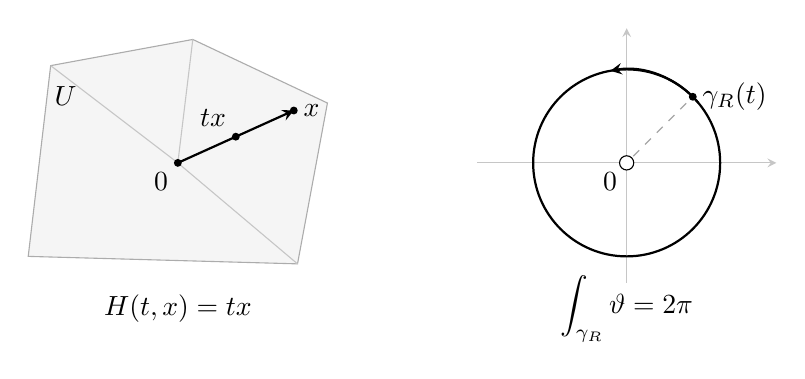
\begin{tikzpicture}[>=stealth,scale=0.95]
		\begin{scope}
			\filldraw[fill=gray!8,draw=gray!65] (-2,-1.25)--(-1.7,1.3)--(0.2,1.65)--(2,0.8)--(1.6,-1.35)--cycle;
			\node at (-1.5,0.9) {\(U\)};
			\draw[gray!45] (0,0)--(-1.7,1.3);
			\draw[gray!45] (0,0)--(0.2,1.65);
			\draw[gray!45] (0,0)--(1.6,-1.35);
			\draw[thick,->] (0,0)--(1.55,0.7);
			\fill (0,0) circle (1.5pt) node[below left] {\(0\)};
			\fill (0.775,0.35) circle (1.5pt) node[above left] {\(tx\)};
			\fill (1.55,0.7) circle (1.5pt) node[right] {\(x\)};
			\node at (0,-1.95) {\(H(t,x)=tx\)};
		\end{scope}
		\begin{scope}[xshift=6cm]
			\draw[gray!45,->] (-2,0)--(2,0);
			\draw[gray!45,->] (0,-1.6)--(0,1.8);
			\draw[thick] (0,0) circle (1.25);
			\draw[thick,->] (40:1.25) arc (40:100:1.25);
			\draw[dashed,gray!70] (0.09,0.09)--(45:1.25);
			\filldraw[fill=white,draw=black] (0,0) circle (2.7pt);
			\node[below left] at (0,0) {\(0\)};
			\fill (45:1.25) circle (1.5pt);
			\node[right] at (45:1.25) {\(\gamma_R(t)\)};
			\node at (0,-1.95) {\(\displaystyle\int_{\gamma_R}\vartheta=2\pi\)};
		\end{scope}
	\end{tikzpicture}
	\caption{左图中，从 \(0\) 到 \(x\) 的径向路径始终留在星形区域内，因此可以沿这一族路径构造原形式。右图的原点被删去，径向收缩不能到达原点；角形式沿圆周的非零周期进一步证明它没有整体原函数。}
	\label{g1:fig:radial-and-period}
\end{figure}


\cref{g1:fig:radial-and-period}把两种构造放在一起：星形区域中径向同伦始终留在定义域内，而穿孔平面中不能把终点设为被删除的原点。穿孔平面上的非恰当性由上面的周期计算证明，不能仅凭一个选定的径向构造失效便作判断。

\ProseParagraphBreak

将角形式限制到单位圆周也得到一个反例。以下取 \(S^1=\{(x,y):x^2+y^2=1\}\)，令 \(j:S^1\hookrightarrow P\) 为包含映射，并记
\[
	\sigma=j^*\vartheta,\qquad
	q:\mathbb R\longrightarrow S^1,\quad q(t)=(\cos t,\sin t).
\]
于是 \(q^*\sigma=\mathrm{d}t\)，沿正向一周的周期为 \(2\pi\)，故 \(\sigma\) 在圆周上不恰当。圆周上的每个一形式都闭，因为二次形式空间为零；所以在一维流形上，闭性本身也不能消除绕圈后的整体障碍。

\begin{proposition}[圆周上的周期判据]
	\label{g1:prop:circle-exactness-period}
	设 \(\lambda\) 为单位圆周 \(S^1\) 上的光滑一形式，写
	\[
		q^*\lambda=a(t)\,\mathrm{d}t,\qquad
		\mathcal P(\lambda)=\int_0^{2\pi}a(t)\,\mathrm{d}t.
	\]
	则 \(a\) 是光滑的 \(2\pi\) 周期函数，且 \(\lambda\) 恰当当且仅当 \(\mathcal P(\lambda)=0\)。更一般地，每个这样的形式都可写成
	\[
		\lambda=c\sigma+\mathrm{d}u,\qquad
		c=\frac{\mathcal P(\lambda)}{2\pi},
	\]
	其中 \(c\) 唯一，光滑函数 \(u:S^1\to\mathbb R\) 在相差常数的意义下唯一。
\end{proposition}
\begin{proof}
	由于 \(q(t+2\pi)=q(t)\) 且 \(q'(t+2\pi)=q'(t)\)，系数 \(a(t)=\lambda_{q(t)}(q'(t))\) 光滑并具有所述周期。若 \(\lambda=\mathrm{d}u\)，沿 \(q|_{[0,2\pi]}\) 使用\cref{g1:lem:exact-path-period}，得到 \(\mathcal P(\lambda)=0\)。

	反过来，设周期为零，令
	\[
		A(t)=\int_0^t a(s)\,\mathrm{d}s.
	\]
	周期性给出 \(A(t+2\pi)-A(t)=\mathcal P(\lambda)=0\)，所以 \(A\) 也为 \(2\pi\) 周期函数。于是可以定义 \(u(q(t))=A(t)\)：两个实数给出同一圆周点时相差 \(2\pi\) 的整数倍，故这个值与代表无关。

	还须检查下降后的函数光滑。\(q'(t)\) 从不为零，由\cref{g1:thm:inverse-function}，\(q\) 在每点附近到一个圆周小弧是微分同胚；在这个小弧上，\(u\) 就是光滑函数 \(A\) 与光滑局部角坐标的复合。因此 \(u\) 光滑。又有
	\[
		q^*(\mathrm{d}u)=\mathrm{d}(u\circ q)=\mathrm{d}A
		=a(t)\,\mathrm{d}t=q^*\lambda.
	\]
	\(q\) 满射且局部微分同胚，每个圆周切向量都能在某个实数点由其微分得到，所以拉回相等蕴含 \(\mathrm{d}u=\lambda\)。

	对一般 \(\lambda\)，取 \(c=\mathcal P(\lambda)/(2\pi)\)，则 \(\lambda-c\sigma\) 的周期为零，刚才的结论给出所需 \(u\)。若存在另一种分解，取周期便知常系数同为 \(c\)；随后两个原函数之差的微分为零。圆周连通，局部常值结论使它们只差常数。
\end{proof}

例如 \(\sigma\) 没有整体原函数，但 \(x\sigma\) 有：在角参数中，它的拉回为 \(\cos t\,\mathrm{d}t=\mathrm{d}(\sin t)\)，所以 \(x\sigma=\mathrm{d}(y|_{S^1})\)。而 \((1+x)\sigma\) 的周期仍为 \(2\pi\)，不恰当。这里决定能否取整体原函数的是一周累积的周期，而不是形式在某个局部坐标中的系数是否为零。
% 纲要条目排为编号小节标题，并进入目录与书签；说明段仍保留于纲要注释中。

% !TeX root = ../../Book1.tex
% 纲要标题：### 14.3 定向、密度与积分
% 纲要位置：几何学计划纲要.md，第 662 行。
% 正文状态：初稿；尚未正式审核。

% 纲要内容开始
% 
% * 定向线和相容图册
% * 密度及不可定向流形的积分
% * 紧支顶次形式的积分
% * 坐标选择和单位分解无关性
% * 定向映射的换元公式
% 
% 纲要内容结束

\section{定向、密度与积分}
\label{g1:sec:1403}

一个局部公式 \(a(x)\,\mathrm{d}x^1\wedge\cdots\wedge\mathrm{d}x^n\) 很像多元积分中的被积表达式，但换坐标时它带的是行列式，而通常的体积换元带绝对行列式。两者之间的符号差，正是定向要处理的问题。密度保留体积缩放而不保留方向，因此在不可定向流形上也能积分。本节先分清这两种对象，再用单位分解把局部积分拼成整体积分。

\ProseParagraphBreak

本节流形均有限维、Hausdorff、第二可数，可以带边界。积分先对光滑紧支对象定义；非紧流形上的非紧支积分还要另查收敛性。分析方面使用一元微积分基本定理、绝对可积函数的 Fubini 定理，以及下面的欧氏换元定理：若 \(F:U\to V\) 是欧氏开集之间的 \(C^1\) 微分同胚，\(h\) 在 \(V\) 上 Lebesgue 可积，则 \((h\circ F)|\det \mathrm{D}F|\) 在 \(U\) 上可积，且
\begin{equation}\label{g1:eq:euclidean-integration-input}
	\int_U h(F(x))|\det \mathrm{D}F_x|\,\mathrm{d}\lambda(x)=\int_V h(y)\,\mathrm{d}\lambda(y).
\end{equation}
这里 \(\lambda\) 是欧氏体积测度，\(\mathrm{d}\lambda\) 没有定向符号。这些是所调用的多元分析基础，分析背景的阅读位置为\cite[Appendix C, Multiple Integrals, pp. 649--655]{Lee2012Smooth}。在半空间图中，对内部应用这些结果；边界超平面是零测集，因而不影响顶维积分。紧支光滑系数有界，其支集位于有限个有界坐标片内，保证下文所用积分绝对收敛。

\subsection{定向线和相容图册}
\label{g1:subsec:1403:01}

回顾\cref{g1:def:determinant-density-line}：当 \(n\geq1\) 时，有序基之间按换基行列式为正划分为两个定向类。在流形上逐点任选一个类还不够，选择必须在局部保持一致。沿小邻域连续移动一个正向标架时，不能突然把它改称反向。

\begin{definition}
	\label{g1:def:manifold-orientation}
	设 \(M\) 为 \(n\geq1\) 维光滑流形。若在每个 \(\mathrm{T}_pM\) 上选定一个定向，并且每点附近存在在各点都为正向的光滑标架，则称这个选择为 \(M\) 的\term[liuxingdingxiang]{定向}[orientation]。允许这样的选择时称 \(M\) 可定向，连同一个选择时称为定向流形。零维流形的定向约定为在每个点选一个符号 \(\varepsilon_p\in\{1,-1\}\)；它用于给有向端点的积分赋号。
\end{definition}

在坐标图 \(x\) 上，令 \(\varepsilon_x(p)\) 表示坐标标架 \((\partial_{x^1},\ldots,\partial_{x^n})\) 是否正向：正向时为 \(1\)，反向时为 \(-1\)。局部一致性等价于 \(\varepsilon_x\) 局部常值。我们通常把图域取为连通的，于是它是一个常数。在两图重叠处，链式法则给出
\begin{equation}\label{g1:eq:orientation-chart-sign}
	\varepsilon_y=\varepsilon_x\operatorname{sgn}\det\frac{\partial x}{\partial y}.
\end{equation}
在无边界情形，必要时反射一个坐标，便可使每张图都正向；于是定向等价于过渡映射的 Jacobian 行列式均为正的相容图册。对于边界模型 \(x^n\geq0\)，保留带符号的表达更方便。尤其在一维区间右端点，只能用向内增大的半直线坐标，不能既要求它正向又要求其取值非负；\(\varepsilon_x\) 会准确记录这个符号。

\ProseParagraphBreak

还可以把符号的变化组织成一个丛。在每张图上取一个实线生成元 \(o_x\)，在交叠处规定
\[
	o_y=\operatorname{sgn}\det\frac{\partial x}{\partial y}\,o_x.
\]
行列式乘法保证三重交叠的余循环条件，所以\cref{g1:thm:bundle-cocycle-gluing}的粘合构造给出一条实光滑线丛，称为\term[dingxiangxian]{定向线丛}[orientation line bundle]，记为 \(\mathfrak o_M\)。它只记录行列式的符号，与使用整个行列式的行列式线丛不同。定向等价于在此线丛中连续选择 \(\pm o_x\) 的一个：表达为 \(\varepsilon_xo_x\)，\eqref{g1:eq:orientation-chart-sign}恰好保证它在换图后不变。零维时取平凡实线丛，在各点选择其正或负单位元。

\begin{proposition}[定向与顶次形式]
	\label{g1:prop:orientation-nonvanishing-form}
	设 \(M\) 为上述光滑 \(n\) 维流形。\(M\) 可定向当且仅当存在处处非零的光滑 \(n\) 形式。给定定向后，可以选择在每个正向有序基上取正值的顶次形式；零维时这表示函数在每点的符号与所选定向一致。
\end{proposition}
\begin{proof}
	对 \(n\geq1\)，若 \(\nu\) 处处非零，就把满足 \(\nu_p(e_1,\ldots,e_n)>0\) 的基规定为正向。局部坐标中 \(\nu=a(x)\,\mathrm{d}x^1\wedge\cdots\wedge\mathrm{d}x^n\)，系数连续且不为零，其符号局部不变，所以确实给出定向。

	反向，\cref{g1:thm:bundle-metric-existence}在 \(\mathrm{T}M\) 上给出光滑正定度量。每张图内把正向标架作光滑正交归一化，正向正交标架之间的矩阵属于 \(\operatorname{SO}(n)\)，行列式为一。因此各正向正交标架的顶次对偶楔积在交叠处相同，粘成所需 \(\nu\)。这也是\cref{g1:prop:orientation-volume-reductions}用于切丛的具体情形。零维时取函数 \(\nu(p)=\varepsilon_p\)；零维流形离散，故它光滑且处处非零。
\end{proof}

例如开 Möbius 带可写成 \(\mathbb R\times(-1,1)\) 在 \((t,u)\sim(t+1,-u)\) 下的商。若它有非零顶次形式，拉回到条带必为 \(a(t,u)\,\mathrm{d}t\wedge\mathrm{d}u\)，且不变性要求
\[
	a(t+1,-u)=-a(t,u).
\]
在中线上，\(a(t+1,0)=-a(t,0)\)，连续性迫使它在一圈中经过零，矛盾。这里每个小矩形都能定向，阻碍来自绕过整个带后的符号变化。

\subsection{密度及不可定向流形的积分}
\label{g1:subsec:1403:02}

\cref{g1:def:determinant-density-line}把密度定义为有序基上的实值函数，换基时乘 \(|\det A|\)。逐点使用这一构造得到密度线丛 \(\mathcal D(M)=|\Lambda^n\mathrm{T}^*M|\)。在坐标图中，光滑密度写为
\[
	\mu=m_x(x)\,|\mathrm{d}x^1\cdots\mathrm{d}x^n|,
\]
换成 \(y\) 坐标后，系数满足
\begin{equation}\label{g1:eq:density-coordinate-change}
	m_y(y)=m_x(x(y))\left|\det\frac{\partial x}{\partial y}\right|.
\end{equation}
系数可以为负，密度线仍是实线性空间；正密度才要求 \(m_x>0\)。若一条光滑密度的支集紧且包含于图域 \(U\)，定义它在该图中的积分为
\[
	I_x(\mu)=\int_{x(U)}m_x(x)\,\mathrm{d}\lambda(x).
\]
由\eqref{g1:eq:density-coordinate-change}和欧氏换元公式，这个数在另一张包含支集的图中不变。这里恰好需要绝对行列式，所以不必指定两图是否同向。

\ProseParagraphBreak

若支集不能放在一张图里，选从属于坐标覆盖的非负光滑单位分解 \(\{\rho_i\}\)，并取 \(\operatorname{supp}\rho_i\subset U_i\)。设 \(\mu\) 紧支，则 \(\rho_i\mu\) 的支集是 \(U_i\) 中的紧集。局部有限性还使只有有限个 \(\rho_i\mu\) 不为零：用有限个局部有限邻域覆盖 \(\operatorname{supp}\mu\)，它们总共只遇到有限个支集。于是可以提出整体积分的定义
\begin{equation}\label{g1:eq:density-integral-definition}
	\int_M\mu=\sum_i I_{x_i}(\rho_i\mu).
\end{equation}
这项和式与单位分解无关的证明，将与顶次形式一起在\subsecref{g1:subsec:1403:04}给出；目前求和的各项和有限性都已经有定义。

\begin{example}[Möbius 带上的面积]
	\label{g1:exm:mobius-density-integral}
	在闭条带 \(\mathbb R\times[-1,1]\) 的上述商上，\(|\mathrm{d}t\,\mathrm{d}u|\) 被变换 \((t,u)\mapsto(t+1,-u)\) 保持，因此下降为正光滑密度。用 \(0\leq t\leq1\)、\(-1\leq u\leq1\) 作基本区域，其积分为 \(2\)。计算时可以把基本区域划成落在商坐标图中的小矩形；公共边以及识别的两条竖边都是二维零测集，不会被重复计入面积。带边界的这个 Möbius 带仍不可定向，因为前面的中线论证不变，却有良定义的面积。
\end{example}

密度解决了测量体积的问题，却不自行产生一个与外微分相容的带符号边界公式。后面的 Stokes 定理仍对定向流形上的微分形式陈述，不能因密度总能积分就删去定向条件。

\subsection{紧支顶次形式的积分}
\label{g1:subsec:1403:03}

现在给 \(M\) 选定定向。若 \(\omega\in\Omega_c^n(M)\) 的支集在一个连通图域 \(U\) 中，并写成
\[
	\omega=a_x(x)\,\mathrm{d}x^1\wedge\cdots\wedge\mathrm{d}x^n,
\]
定义
\begin{equation}\label{g1:eq:oriented-chart-integral}
	I_x^{\mathrm{or}}(\omega)=\varepsilon_x\int_{x(U)}a_x(x)\,\mathrm{d}\lambda(x).
\end{equation}
在正向图中 \(\varepsilon_x=1\)，得到熟悉的公式；反向图中要额外乘 \(-1\)。这不是对被积系数取绝对值，形式的积分可以为负，也可以因正负部分抵消而为零。

\ProseParagraphBreak

对一般紧支顶次形式，以从属于坐标覆盖的单位分解规定
\begin{equation}\label{g1:eq:top-form-integral-definition}
	\int_M\omega=\sum_i I_{x_i}^{\mathrm{or}}(\rho_i\omega).
\end{equation}
和式仍只有有限个非零项。零维流形上的紧集只有有限个点，此时 \(0\) 形式就是函数，定义专门写为
\[
	\int_M f=\sum_{p\in M}\varepsilon_p f(p),
\]
其中紧支性保证求和有限。特别地，一个正向点的积分为函数值，负向点的积分为其相反数。这将使区间的两个边界端点分别贡献 \(f(b)\) 与 \(-f(a)\)。

\ProseParagraphBreak

定向也给出顶次形式到密度的线性对应。令 \(S_o\omega\) 在 \(x\) 图中的密度系数为 \(\varepsilon_xa_x\)。因为
\[
	a_y=a_x\det\frac{\partial x}{\partial y},\qquad
	\varepsilon_y=\varepsilon_x\operatorname{sgn}\det\frac{\partial x}{\partial y},
\]
乘积 \(\varepsilon_ya_y\) 恰按绝对行列式变换，所以这些局部系数粘成密度。这与非线性的 \(|\omega|\) 不同：\(S_o\omega\) 保留相对于给定定向的正负号，\(|\omega|\) 只保留绝对大小。由局部定义，\(\int_M\omega=\int_M S_o\omega\)。反转定向时 \(S_o\) 变号，故形式积分也变号，密度积分本身则不变。

\subsection{坐标选择和单位分解无关性}
\label{g1:subsec:1403:04}

\begin{theorem}[流形积分的良定义性]
	\label{g1:thm:integral-well-defined}
	设 \(M\) 为有限维、Hausdorff、第二可数光滑流形，允许边界。\eqref{g1:eq:density-integral-definition}对每个紧支光滑密度定义一个与坐标覆盖和从属单位分解无关的实数。若另给定向，则\eqref{g1:eq:top-form-integral-definition}对每个紧支光滑顶次形式也有同样性质。两种积分均线性；非负且不恒为零的光滑密度积分严格为正。
\end{theorem}
\begin{proof}
	密度在一张图中的积分已经由欧氏换元证明与图无关。形式也如此：在两个图的交中，其系数相差有符号行列式，图的定向符号满足\eqref{g1:eq:orientation-chart-sign}。两者相乘得到绝对行列式，故
	\[
		\varepsilon_y\int a_y\,\mathrm{d}\lambda(y)
		=\varepsilon_x\int a_x(x(y))\left|\det\frac{\partial x}{\partial y}\right|\mathrm{d}\lambda(y)
		=\varepsilon_x\int a_x\,\mathrm{d}\lambda(x).
	\]
	若交集不连通，对各连通分支使用相同公式，或直接把局部常值符号保留在被积函数中。边界图的换元在内部进行，边界零测不改变结果。

	现取两套从属于坐标覆盖的单位分解 \(\{\rho_i\}\)、\(\{\sigma_j\}\)，图分别记为 \(x_i,y_j\)。令 \(u\) 表示待积的密度或顶次形式。只有有限个支集与 \(\operatorname{supp}u\) 相交，因此下面实为有限次拆分：
	\[
		\sum_i I_{x_i}(\rho_i u)
		=\sum_{i,j}I_{x_i}(\rho_i\sigma_j u)
		=\sum_{i,j}I_{y_j}(\rho_i\sigma_j u)
		=\sum_j I_{y_j}(\sigma_j u).
	\]
	形式情形中的 \(I\) 理解为 \(I^{\mathrm{or}}\)。中间每个对象的支集紧且包含在 \(U_i\cap V_j\) 中，所以第一步的单图换元确实适用。最外两次等式分别使用 \(\sum_j\sigma_j=1\)、\(\sum_i\rho_i=1\)，并利用欧氏积分的线性。由此同时排除了覆盖、坐标与单位分解的选择依赖。

	线性可以在同一套覆盖和单位分解中逐项验证。若 \(\mu\geq0\) 且某点处严格为正，连续性给出某张图内的一块区域，其系数有正下界。该点处至少一个 \(\rho_i>0\)，缩小区域后 \(\rho_i\mu\) 的系数仍有正下界，因此这一项积分正，其余项非负。边界点附近可取正体积的半球内部，零维时则是一项正数。这证明严格正性。
\end{proof}

证明中的共同细化 \(\rho_i\sigma_j\) 是关键：不必在两套坐标之间直接比较整个和式，只需把它们拆成同时落在两张图中的小块。局部有限性让这一分解在紧支集上化为有限运算，避免了任何未经说明的无穷级数换序。

\begin{proposition}[度量的体积积分]
	\label{g1:prop:metric-volume-integration}
	设 \(g\) 为 \(M^n\) 上的光滑正定度量。其正体积密度在坐标中为
	\[
		\mu_g=\sqrt{\det(g_{ij})}\,|\mathrm{d}x^1\cdots\mathrm{d}x^n|.
	\]
	若 \(M\) 定向，则相应的正体积形式为
	\[
		\operatorname{vol}_g=\varepsilon_x\sqrt{\det(g_{ij})}\,\mathrm{d}x^1\wedge\cdots\wedge\mathrm{d}x^n,
	\]
	并且对每个紧支光滑函数 \(f\)，有 \(\int_M f\operatorname{vol}_g=\int_M f\mu_g\)。
\end{proposition}
\begin{proof}
	\cref{g1:prop:gram-volume-density}在每个切空间给出 \(\mu_g(e)=\sqrt{\det[g(e_i,e_j)]}\)，取坐标标架就得到密度公式；正定性使行列式正，其正平方根随点光滑。把坐标标架的定向符号乘入顶次形式，便使其在正向标架上取正值，且换图时相容。最后 \(S_o(f\operatorname{vol}_g)\) 的局部系数为 \(f\sqrt{\det(g_{ij})}\)，正是 \(f\mu_g\)，所以积分相同。
\end{proof}

例如平面的极坐标在 \(r>0\) 的角度分支上给出 \(g=\mathrm{d}r^2+r^2\mathrm{d}\theta^2\)，所以体积密度为 \(r|\mathrm{d}r\,\mathrm{d}\theta|\)。\(r=0\) 不是这张坐标图的一点，不能把极坐标表达在原点的退化误认为欧氏度量退化。对半径为 \(R\) 的圆盘积分得到 \(\int_0^{2\pi}\int_0^R r\,\mathrm{d}r\,\mathrm{d}\theta=\pi R^2\)；被忽略的中心及切开的射线面积为零。

\subsection{定向映射的换元公式}
\label{g1:subsec:1403:05}

对任意光滑映射都能拉回微分形式，但积分的简单换元公式首先适用于微分同胚。非单射映射可能重复覆盖区域，微分降秩也可能压缩维数；这些情况不能仅凭拉回有定义就沿用同一个积分等式。

\begin{theorem}[定向换元]
	\label{g1:thm:oriented-change-variables}
	设 \(F:M^n\to N^n\) 为光滑流形之间的微分同胚，允许边界。
	\begin{enumerate}
		\item 对 \(N\) 上的紧支光滑密度 \(\mu\)，其微分同胚拉回满足 \(\int_M F^*\mu=\int_N\mu\)。
		\item 若两流形定向，定义 \(s_F(p)=1\) 当 \(\mathrm{d}F_p\) 保定向，反向时为 \(-1\)。则 \(s_F\) 局部常值，且对任意 \(\omega\in\Omega_c^n(N)\)，
		\[
			\int_M F^*\omega=\int_N(s_F\circ F^{-1})\omega.
		\]
		特别地，整体保定向时积分不变，整体反定向时积分变号。若 \(M\) 连通，符号只有上述两种整体可能。
	\end{enumerate}
	零维时，用源点和像点的定向符号之比定义 \(s_F\)，同一公式成立。
\end{theorem}
\begin{proof}
	微分同胚将紧集的原像变为紧集，所以两种拉回仍紧支。对目标支集选有限个所需坐标片及从属单位分解，再拉回到源；它们的拉回仍构成从属单位分解。故只需证明单图的结果。

	在源图 \(x\) 和目标图 \(y\) 中，记 \(G=y\circ F\circ x^{-1}\)。若 \(\mu=m(y)|\mathrm{d}y^1\cdots\mathrm{d}y^n|\)，则其拉回系数为 \(m(G(x))|\det \mathrm{D}G_x|\)，欧氏换元直接给出第一项。若 \(\omega=a(y)\,\mathrm{d}y^1\wedge\cdots\wedge\mathrm{d}y^n\)，则拉回系数为 \(a(G(x))\det \mathrm{D}G_x\)。源、目标图的定向符号分别为 \(\varepsilon_x,\varepsilon_y\)，有
	\[
		s_F=\varepsilon_x\varepsilon_y\operatorname{sgn}\det \mathrm{D}G,
	\]
	所以 \(\varepsilon_x\det \mathrm{D}G=s_F\varepsilon_y|\det \mathrm{D}G|\)。代入单图积分，再用欧氏换元，便得到第二项；逐片相加完成证明。符号的局部常值性来自非零行列式的连续性，在连通流形上因此恒定。零维公式就是把有限项求和按双射重新编号。
\end{proof}

以反射 \(F(x^1,x^2)=(-x^1,x^2)\) 为例，在标准定向的平面上，\(F^*(a\,\mathrm{d}x^1\wedge\mathrm{d}x^2)=-a(-x^1,x^2)\,\mathrm{d}x^1\wedge\mathrm{d}x^2\)，故紧支形式的积分变号；密度的拉回则没有这个负号。又如圆周映射 \(e^{\mathrm{i}\theta}\mapsto e^{2\mathrm{i}\theta}\) 不是微分同胚，它把角形式拉回为两倍，积分也变成两倍。后者涉及重复覆盖次数，将在\secref{g1:sec:1405}进一步说明，不能当作当前换元定理的一个无条件推论。

% 纲要条目排为编号小节标题，并进入目录与书签；说明段仍保留于纲要注释中。

% !TeX root = ../../Book1.tex
% 纲要标题：### 14.4 边界定向与 Stokes 的证明
% 纲要位置：几何学计划纲要.md，第 670 行。
% 正文状态：初稿；尚未正式审核。

% 纲要内容开始
% 
% * 外法向优先的边界约定
% * 半空间中的局部公式
% * 通过单位分解粘合
% * 带角区域及逐项边界符号
% * Green、Gauss 公式作为特例
% 
% 纲要内容结束

\section{边界定向与 Stokes 的证明}
\label{g1:sec:1404}

在一元微积分中，导数的积分只留下区间两个端点的函数值，而且右端点取正号、左端点取负号。Stokes 定理把这个关系推广到微分形式：区域内部的外微分积分，等于边界上原形式的积分。这里“边界”必须带有由区域定向确定的方向，否则等式连符号都不能确定。

\ProseParagraphBreak

第九章已经在曲面坐标中证明了所需的 Green 公式，并据此把联络形式的边界积分换成曲率积分，见\cref{g1:lem:green-formula,g1:thm:local-gauss-bonnet}。本节从同一个积分基本定理出发，先处理任意维半空间，再用第十二章的光滑单位分解得到整体公式。所有形式都光滑至边界；非紧流形上的形式要求紧支，支集可以接触实际边界。

\subsection{外法向优先的边界约定}
\label{g1:subsec:1404:01}

设 \(M^n\) 为有向带边界光滑流形，\(n\ge1\)，包含映射记为 \(j:\partial M\hookrightarrow M\)。\cref{g1:prop:boundary-chart-invariance}说明，\(\partial M\) 本身是 \(n-1\) 维无边界光滑流形；其完整切空间由边界坐标中最后一个分量为零的向量组成。若在边界图中把 \(M\) 写成 \(x^n\ge0\)，则指向外侧的横截向量满足 \(\mathrm{d}x^n(\nu)<0\)。这个描述只用边界两侧的区分，不需要长度或正交关系。

\begin{definition}[边界定向]\label{g1:def:boundary-orientation}
	设 \(M^n\) 为有向带边界光滑流形，\(n\ge1\)。在 \(p\in\partial M\) 取一个外向横截向量 \(\nu\)，即在边界定义坐标 \(\rho\ge0\) 下满足 \(\mathrm{d}\rho_p(\nu)<0\)。边界取\term[waifaxiangyouxian]{外法向优先}[outward-normal-first]的定向：当 \(n\ge2\) 时，基 \((v_1,\ldots,v_{n-1})\) 在 \(\mathrm{T}_p\partial M\) 中为正向，当且仅当
	\[
		(\nu,v_1,\ldots,v_{n-1})
	\]
	在 \(\mathrm{T}_pM\) 中为正向。等价地，若 \(\Omega_p\) 是表示 \(M\) 正定向的非零顶次协变向量，则 \((\iota_\nu\Omega_p)|_{\mathrm{T}_p\partial M}\) 表示边界的正定向。后一表述也适用于 \(n=1\)：它给边界点指定一个正负号。
\end{definition}

名称中的“法向”只指横截方向；若另有黎曼度量，才可以特选外向单位法向。先核对这个约定不依赖选择。两种边界定义坐标 \(\rho,\rho'\) 在边界上都为零，局部可写成
\[
	\rho'=\rho\,a,\qquad
	a(x',\rho)=\int_0^1\partial_\rho\rho'(x',t\rho)\,\mathrm{d}t.
\]
边界坐标变换可逆，且把内侧映到内侧，所以 \(a(p)>0\)：其边界处的法向导数不为零，又不能为负。这也可由\cref{g1:prop:boundary-smooth-derivative}的链式法则和一侧非负性直接判断。因此 \(\mathrm{d}\rho'_p=a(p)\mathrm{d}\rho_p\)，外向条件与坐标无关。

\ProseParagraphBreak

若 \(\nu,\nu'\) 都外向，则在一维商空间 \(\mathrm{T}_pM/\mathrm{T}_p\partial M\) 中，它们位于同一条半直线上，故
\[
	\nu'=c\nu+w,\qquad c>0,\quad w\in \mathrm{T}_p\partial M.
\]
把第一列由 \(\nu\) 换为 \(\nu'\)，行列式只乘以正数 \(c\)，因为 \(w\) 是其余切向列的线性组合。等价地，插入 \(w\) 后限制到边界切空间的顶次形式为零。因此边界定向与外向横截向量及正顶次形式的选择无关，且随点光滑变化。

在标准定向半空间
\[
	H^n=\{x^n\ge0\},\qquad
	\Omega=\mathrm{d}x^1\wedge\cdots\wedge\mathrm{d}x^n
\]
中，可以取 \(\nu=-\partial_{x^n}\)。于是
\begin{equation}\label{g1:eq:half-space-boundary-orientation}
	\left.\iota_{-\partial_{x^n}}\Omega\right|_{\partial H^n}
	=(-1)^n\,\mathrm{d}x^1\wedge\cdots\wedge\mathrm{d}x^{n-1}.
\end{equation}
所以边界坐标 \((x^1,\ldots,x^{n-1})\) 的通常定向，与诱导边界定向相差 \((-1)^n\)。这个符号来自把最后一个坐标向量移到第一位，再乘上外向向量的负号。

\ProseParagraphBreak

当 \(n=1\) 时，标准半直线的边界点 \(0\) 取负号；对按递增参数定向的区间 \([a,b]\)，左端点取负、右端点取正。按照上一节的有向零维积分约定，
\[
	\int_{\partial[a,b]}f=f(b)-f(a).
\]
零维流形另约定边界为空，不再应用“降低一维”的基向量描述。此时没有需要讨论的负一次形式；若记 \(\Omega^{-1}=0\)，Stokes 等式只表示 \(0=0\)。

\subsection{半空间中的局部公式}
\label{g1:subsec:1404:02}

高维公式的局部计算只多了一个排列符号。把一般 \(n-1\) 次形式按“缺少哪个坐标微分”分组，并在第 \(i\) 项预先放入 \((-1)^{i-1}\)，可以让外微分后的各项都具有相同正号。以下用帽子表示删去相应因子。

\begin{lemma}[半空间中的 Stokes 公式]\label{g1:lem:half-space-stokes}
	设 \(n\ge1\)，\(H^n=\{x^n\ge0\}\) 取标准定向，边界取外法向优先定向。若 \(\alpha\) 是 \(H^n\) 上光滑至边界的紧支 \(n-1\) 次形式，则
	\[
		\int_{H^n}\mathrm{d}\alpha=\int_{\partial H^n}j^*\alpha.
	\]
	在无边界模型 \(\mathbb R^n\) 上，任意紧支光滑 \(n-1\) 次形式都满足 \(\int_{\mathbb R^n}\mathrm{d}\alpha=0\)。紧支集允许与 \(x^n=0\) 相交。
\end{lemma}
\begin{proof}
	唯一写成
	\[
		\alpha=\sum_{i=1}^n(-1)^{i-1}a_i(x)\,
		\mathrm{d}x^1\wedge\cdots\wedge\widehat{\mathrm{d}x^i}\wedge\cdots\wedge\mathrm{d}x^n.
	\]
	每个 \(a_i\) 光滑且紧支。由\cref{g1:thm:exterior-derivative}的坐标公式，求外微分时，只有 \(\partial_i a_i\,\mathrm{d}x^i\) 那一项不因重复微分而消失。把 \(\mathrm{d}x^i\) 移到第 \(i\) 位又产生 \((-1)^{i-1}\)，两个符号抵消，故
	\begin{equation}\label{g1:eq:stokes-local-divergence}
		\mathrm{d}\alpha=\left(\sum_{i=1}^n\partial_i a_i\right)
		\mathrm{d}x^1\wedge\cdots\wedge\mathrm{d}x^n.
	\end{equation}

	取 \(R\) 足够大，使全部系数支集位于 \((-R,R)^{n-1}\times[0,R)\)。连续系数及其导数在这个紧盒上可积，累次积分的 Fubini 公式允许先沿任一坐标积分。对 \(i<n\)，沿 \(x^i\) 的积分区间两端，\(a_i\) 都为零，所以
	\[
		\int_{H^n}\partial_i a_i\,\mathrm{d}x=0.
	\]
	最后一个坐标则从零开始，积分基本定理给出
	\[
		\int_{H^n}\partial_n a_n\,\mathrm{d}x
		=-\int_{\mathbb R^{n-1}}a_n(x',0)\,\mathrm{d}x'.
	\]
	因此体积分只留下这一个负的边界值。

	在边界上拉回时，含 \(\mathrm{d}x^n\) 的项全部消失，故
	\[
		j^*\alpha=(-1)^{n-1}a_n(x',0)\,
		\mathrm{d}x^1\wedge\cdots\wedge\mathrm{d}x^{n-1}.
	\]
	但边界的定向符号还要乘上\eqref{g1:eq:half-space-boundary-orientation}中的 \((-1)^n\)。于是
	\[
		\int_{\partial H^n}j^*\alpha
		=(-1)^n(-1)^{n-1}\int_{\mathbb R^{n-1}}a_n(x',0)\,\mathrm{d}x'
		=-\int_{\mathbb R^{n-1}}a_n(x',0)\,\mathrm{d}x',
	\]
	恰与体积分相同。\(n=1\) 时，右侧按零维积分解释为 \(-a_1(0)\)，同样成立。

	在 \(\mathbb R^n\) 上，每个坐标都在完整实轴上积分，紧支性使各方向两端的系数为零，故所有偏导积分都为零。
\end{proof}

这里没有把 \(\alpha\) 越过实际边界 \(x^n=0\) 补成零。那样补零通常不光滑，而且会错误地抹掉边界项。紧支性只保证在足够远的辅助截断边缘处系数为零，真正的边界值 \(a_n(x',0)\) 完整保留。

\subsection{通过单位分解粘合}
\label{g1:subsec:1404:03}

\begin{theorem}[Stokes 定理]\label{g1:thm:stokes}
	设 \(M^n\) 为有限维、Hausdorff、第二可数的有向光滑流形，允许有边界，\(n\ge1\)。给 \(\partial M\) 外法向优先定向，记包含映射为 \(j\)。对每个紧支光滑 \(n-1\) 次形式 \(\omega\in\Omega_c^{n-1}(M)\)，有
	\begin{equation}\label{g1:eq:stokes}
		\int_M\mathrm{d}\omega=\int_{\partial M}j^*\omega.
	\end{equation}
	此式称为\term[stokesdingli]{Stokes 定理}[Stokes theorem]。不要求 \(M\) 紧；若 \(M\) 紧，则任意光滑 \(n-1\) 次形式自动满足支集条件。
\end{theorem}
\begin{proof}
	令 \(K=\operatorname{supp}\omega\)。在 \(M\setminus K\) 的每个点附近，\(\omega\) 恒为零，故 \(\operatorname{supp}\mathrm{d}\omega\subseteq K\)。由于边界是闭集，\(j^*\omega\) 的支集包含于紧集 \(K\cap\partial M\)。因此两边的积分均在上一节已定义的紧支积分范围内。

	用内部坐标图和边界坐标图覆盖 \(M\)，再由\cref{g1:thm:smooth-partition-unity}取从属光滑单位分解 \(\{\rho_i\}\)。局部有限的支集族只会有有限个成员与紧集 \(K\) 相交：给 \(K\) 中每一点选一个只遇到有限个支集的邻域，再从这些邻域取有限子覆盖即可。因此
	\[
		\omega=\sum_i\omega_i,\qquad \omega_i=\rho_i\omega
	\]
	实际上只有有限个非零项；每个 \(\omega_i\) 的支集是位于对应图域 \(U_i\) 内的紧集。

	将 \(\omega_i\) 写入坐标。其坐标支集紧含于相对开图域，故可越过这个图域的人为边缘补零到整个 \(\mathbb R^n\) 或 \(H^n\)，而保持光滑；补零没有越过 \(H^n\) 的实际边界。由\cref{g1:prop:exterior-pullback}，坐标拉回与外微分交换。对补零形式应用\cref{g1:lem:half-space-stokes}，再用\cref{g1:thm:oriented-change-variables}把积分搬回，便得
	\[
		\int_M\mathrm{d}\omega_i=\int_{\partial M}j^*\omega_i.
	\]
	这里任一图都可以带有定向符号 \(\varepsilon_i=\pm1\)：若坐标参数化反向，体积分和它诱导的边界积分同时乘以 \(-1\)，所以局部等式仍成立。特别是在一维右端点附近，无须强行要求到标准半直线的坐标正向。

	最后把有限个等式相加。注意局部公式作用于 \(\mathrm{d}(\rho_i\omega)\)，而不是直接作用于 \(\rho_i\mathrm{d}\omega\)；乘积法则产生的项正好消去：
	\[
		\begin{aligned}
			\sum_i\mathrm{d}(\rho_i\omega)
			&=\sum_i\mathrm{d}\rho_i\wedge\omega+\sum_i\rho_i\,\mathrm{d}\omega\\
			&=\mathrm{d}\!\left(\sum_i\rho_i\right)\wedge\omega+\mathrm{d}\omega
			=\mathrm{d}\omega.
		\end{aligned}
	\]
	这些等式可先按局部有限和理解，而乘上 \(\omega\) 后只有前述有限个非零项。边界上的和同样为 \(j^*\omega\)。积分的线性及\cref{g1:thm:integral-well-defined}的坐标、单位分解无关性遂给出\eqref{g1:eq:stokes}。
\end{proof}

若 \(M\) 无边界，结论是 \(\int_M\mathrm{d}\omega=0\)；若 \(M=[a,b]\)，结论就是积分基本定理。非紧情形的紧支要求控制了“远处的边界”：仅仅知道 \(\mathrm{d}\omega\) 的积分收敛，并不能保证无穷远没有留下额外项，习题中会给出一维例子。

\subsection{带角区域及逐项边界符号}
\label{g1:subsec:1404:04}

矩形和单形在角点处不具有半空间局部模型。这里先明确所讨论的对象，再把局部公式推广到正交象限；角棱不贡献新的积分项，但邻接的每张面都必须保留。

\begin{definition}[带角流形]\label{g1:def:manifold-with-corners}
	一个 \(n\) 维\term[daijiaoliuxing]{带角流形}[manifold with corners]是 Hausdorff、第二可数空间，带有到
	\[
		Q_k^n=[0,\infty)^k\times\mathbb R^{n-k},
		\qquad 0\le k\le n
	\]
	的相对开集的坐标图；换坐标及其逆都要求局部延拓为欧氏空间中的光滑映射。函数、微分形式和定向也按这种局部延拓定义。在一点附近，只保留在那里取零的受限坐标，其个数称为该点的深度；深度一部分是光滑的余维一边界，深度至少二的部分称为角棱。
\end{definition}

这个深度与坐标无关。像第十一章半空间的论证一样，局部延拓的导数由内部稠密性唯一确定，互逆变换的导数互逆。在深度 \(k\) 的点，单侧曲线的速度构成锥
\[
	C_p=\{v:v^1,\ldots,v^k\ge0\},
\]
其最大线性子空间 \(C_p\cap(-C_p)\) 的维数为 \(n-k\)。坐标变换的微分把这个速度锥同构到目标的速度锥，因此保持 \(k\)。深度一部分在小坐标邻域内分成 \(k\) 张局部面 \(x^i=0\) 的内部；换坐标保持深度，并把这些连通的局部面分支一一对应。每张面的定向先在深度一点由外法向优先确定，再连续延伸到它的角棱。

\ProseParagraphBreak

顶次积分沿用上一节的坐标定义。正交象限中边界在 \(n\) 维测度下为零，不影响体积分；对每张余维一面，角棱在该面内的 \(n-1\) 维测度也为零，因为它们在面坐标中是一个或多个坐标取零的集合。因此边界积分按每张局部面分别计算，同一角点邻接的不同面各计一次，而不把整个拓扑边界误认为一张光滑流形。

\ProseParagraphBreak

这些面上的积分与坐标选择相容：在深度一部分应用有向换元公式即可。若某积分的支集接触角棱，可以先去掉面坐标中宽度为 \(\varepsilon\) 的角棱条带，再令 \(\varepsilon\downarrow0\)。在所用紧坐标片内，形式系数与换元 Jacobian 有界，条带体积趋于零，遗漏积分的绝对值也趋于零。于是普通换元公式延续到接触角棱的积分。用有限坐标分解求和时，两种分解可通过权重乘积作共同细化，逐面利用换元和权重总和为 \(1\)，证明边界积分不依赖分解。以下的 \(\int_{\partial M}\omega\) 就表示这种按局部面分支计算的积分；面上的形式均指包含拉回。

\begin{theorem}[带角流形上的 Stokes 公式]\label{g1:thm:stokes-corners}
	设 \(M^n\) 为有向、Hausdorff、第二可数的光滑带角流形，\(n\ge1\)，\(\omega\) 为光滑至各面的紧支 \(n-1\) 次形式。各余维一面取外法向优先定向，边界积分按局部面分支计算，则
	\[
		\int_M\mathrm{d}\omega=\int_{\partial M}\omega.
	\]
	余维至少二的角棱不增加独立积分项。
\end{theorem}
\begin{proof}
	先在标准定向的 \(Q_k^n\) 上取紧支形式
	\[
		\alpha=\sum_{i=1}^n(-1)^{i-1}a_i\,
		\mathrm{d}x^1\wedge\cdots\wedge\widehat{\mathrm{d}x^i}\wedge\cdots\wedge\mathrm{d}x^n.
	\]
	外微分仍由\eqref{g1:eq:stokes-local-divergence}给出。对不受限坐标 \(i>k\)，偏导积分为零；对 \(i\le k\)，沿 \([0,\infty)\) 使用积分基本定理，得到
	\[
		\int_{Q_k^n}\mathrm{d}\alpha
		=-\sum_{i=1}^k\int_{F_i}a_i|_{x^i=0}\,\mathrm{d}x^{\widehat i},
		\qquad F_i=Q_k^n\cap\{x^i=0\}.
	\]
	这里右侧暂按其余坐标的递增次序使用通常正测度。面 \(F_i\) 的外向向量为 \(-\partial_{x^i}\)，所以相对于这组面坐标，诱导定向的符号为 \((-1)^i\)。拉回 \(\alpha\) 后只留下 \((-1)^{i-1}a_i\,\mathrm{d}x^{\widehat i}\)，两者相乘正好是 \(-a_i\,\mathrm{d}x^{\widehat i}\)。因此上式就是各有向面的积分之和。各坐标面的相交部分测度为零，不会在这个计算之外再留下角点项。

	现在令 \(K=\operatorname{supp}\omega\)。紧集附近只需有限个坐标截断函数。具体地，在每点的带角坐标中取两层相对球，把\cref{g1:lem:smooth-bump-function}中的欧氏截断函数限制到正交象限，得到支集紧含于外层图域、在内层为 \(1\) 的光滑函数。选有限个内层覆盖 \(K\)，记对应函数为 \(b_1,\ldots,b_N\)。其和 \(b\) 在 \(K\) 的开邻域 \(W\) 上为正，令 \(\rho_i=b_i/b\) 于 \(W\)。于是 \(\sum_i\rho_i=1\) 于 \(W\)。

	在 \(W\) 上取 \(\omega_i=\rho_i\omega\)，再在 \(M\setminus W\) 补零。因为 \(K\subset W\)，每个补零位置附近 \(\omega\) 本来就为零，故 \(\omega_i\) 光滑；其支集位于 \(K\cap\operatorname{supp}b_i\)，是相应图域内的紧集。对各 \(\omega_i\) 使用刚证的象限公式，按图的定向符号搬回，并把有限个等式相加。由 \(\sum_i\omega_i=\omega\)，或等价地由 \(\sum_i\mathrm{d}\rho_i=0\) 于 \(W\)，得到所需整体等式。
\end{proof}

如果一个区域由有限个这样的有向块拼成，并且相邻块沿完整面光滑贴合，就对每块应用公式再相加。公共面的外向横截方向对两块相反，而环境定向相同，所以两次诱导面定向相反，内部面项抵消。这里先按面在各块中出现的次数计入，再作抵消；不能一开始就把同一个几何面只算一次。

\ProseParagraphBreak

对按 \((x^1,\ldots,x^n)\) 定向的矩形 \(R=\prod_{i=1}^n[a_i,b_i]\)，记 \(R_{\widehat i}\) 为删去第 \(i\) 个坐标的矩形，取其剩余坐标递增次序的定向；令 \(\delta_i^+,\delta_i^-\) 分别插入 \(x^i=b_i,a_i\)。上面的向量次序给出：上侧面的外向向量为 \(+\partial_{x^i}\)，符号为 \((-1)^{i-1}\)；下侧面的外向向量为 \(-\partial_{x^i}\)，符号为 \((-1)^i\)。于是
\begin{equation}\label{g1:eq:rectangle-boundary-signs}
	\int_{\partial R}\omega
	=\sum_{i=1}^n(-1)^{i-1}\left(
		\int_{R_{\widehat i}}(\delta_i^+)^*\omega
		-\int_{R_{\widehat i}}(\delta_i^-)^*\omega
	\right).
\end{equation}
若把 \(\omega\) 写成前面的 \(\sum_i(-1)^{i-1}a_i\,\mathrm{d}x^{\widehat i}\)，两组排列符号抵消，留下的正是每个系数“上端值减下端值”。这也从逐坐标的积分基本定理直接验证了矩形公式。

\begin{lemma}[有序单形的边界定向]\label{g1:lem:simplex-boundary-orientation}
	设 \(n\ge1\)。给非退化有序仿射单形 \([v_0,\ldots,v_n]\) 以有序边向量 \((v_1-v_0,\ldots,v_n-v_0)\) 所确定的定向。删去第 \(i\) 个顶点后，面按剩余顶点的原次序定向，则该面的诱导边界定向等于此面定向的 \((-1)^i\) 倍。特别地，对标准单形
	\[
		\Delta^n=\left\{t\in\mathbb R^n:t^j\ge0,\ \sum_{j=1}^nt^j\le1\right\}
		=[0,e_1,\ldots,e_n],
	\]
	令 \(\delta_i:\Delta^{n-1}\to\Delta^n\) 为按该顶点次序参数化第 \(i\) 面的仿射映射。对光滑至边界的 \(n-1\) 次形式 \(\alpha\)，有
	\begin{equation}\label{g1:eq:simplex-stokes}
		\int_{\Delta^n}\mathrm{d}\alpha
		=\sum_{i=0}^n(-1)^i\int_{\Delta^{n-1}}\delta_i^*\alpha.
	\end{equation}
\end{lemma}
\begin{proof}
	先对标准单形计算。对 \(i\ge1\)，第 \(i\) 面为 \(t^i=0\)，删去 \(e_i\) 后的有序边向量为
	\[
		(e_1,\ldots,\widehat e_i,\ldots,e_n).
	\]
	取外向横截向量 \(-e_i\)，则
	\[
		\det(-e_i,e_1,\ldots,\widehat e_i,\ldots,e_n)=(-1)^i.
	\]
	因此该面的边界定向正好是有序面定向的 \((-1)^i\) 倍。

	第零面为 \(\sum_jt^j=1\)，其有序顶点为 \(e_1,\ldots,e_n\)，故有序切向基为
	\[
		(e_2-e_1,\ldots,e_n-e_1).
	\]
	这里可取外向横截向量 \(e_1\)，因为沿它移动会增大 \(\sum_jt^j\)。把第一列加到后面各列，可得
	\[
		\det(e_1,e_2-e_1,\ldots,e_n-e_1)=1.
	\]
	所以第零面的符号为 \(+1=(-1)^0\)。这一步使用横截向量而非必须垂直于面的单位法向，正体现了边界定向的选择无关性。

	一般有序仿射单形由映射 \(t\mapsto v_0+\sum_jt^j(v_j-v_0)\) 从标准单形得到；按题定的定向，它保向，并把各有序面与外向半侧对应，故保持上述符号。标准单形在每一点可用独立的活动面定义函数作为部分坐标，因而是带角流形；对它应用\cref{g1:thm:stokes-corners}即得\eqref{g1:eq:simplex-stokes}。当 \(n=1\) 时，这给出 \([v_1]-[v_0]\)；零维单形则另约定边界为空。
\end{proof}

\subsection{Green、Gauss 公式作为特例}
\label{g1:subsec:1404:05}

先看平面。设 \(D\subset\mathbb R^2\) 为紧的有向光滑带边界区域，或可按上一小节分块处理的带角区域，取标准面积定向；\(P,Q\) 在其邻域光滑。令
\[
	\alpha=P\,\mathrm{d}x+Q\,\mathrm{d}y,\qquad
	\mathrm{d}\alpha=(\partial_xQ-\partial_yP)\,\mathrm{d}x\wedge\mathrm{d}y.
\]
Stokes 公式立即给出
\begin{equation}\label{g1:eq:green-from-stokes}
	\int_{\partial D}P\,\mathrm{d}x+Q\,\mathrm{d}y
	=\int_D(\partial_xQ-\partial_yP)\,\mathrm{d}x\,\mathrm{d}y.
\end{equation}
现在解释边界方向。若 \(\nu\) 为外向单位法向，\(J\) 为平面的正向四分之一转动，则正向单位切向为 \(T=J\nu\)，因为 \((\nu,J\nu)\) 是正向基。行进方向的左侧为 \(JT=-\nu\)，恰好指向区域内部。因此正向边界使区域在左，外圈逆时针，孔洞的边界顺时针，如\cref{g1:fig:boundary-outward-first}。这与第九章的约定一致；\cref{g1:lem:green-formula}还单独证明了该章使用的分片 \(C^2\) 边界、\(C^1\) 一形式版本，并用截角极限处理内角在 \((0,2\pi)\) 内的角点。

% !TeX root = ../Book1.tex
% 外法向优先约定在环域外圈和内圈上的不同方向。
\begin{figure}[htbp]
	\centering
	\begin{tikzpicture}[font=\small,scale=1.05]
		\fill[GeometryBlueLight,even odd rule] (0,0) circle[radius=2] (0,0) circle[radius=0.88];
		\draw[GeometryBlue,thick] (0,0) circle[radius=2];
		\draw[GeometryBlue,thick] (0,0) circle[radius=0.88];
		\draw[GeometryBlue,very thick,->] (110:2) arc[start angle=110,end angle=155,radius=2];
		\draw[GeometryBlue,very thick,->] (245:2) arc[start angle=245,end angle=290,radius=2];
		\draw[GeometryBlue,very thick,->] (150:0.88) arc[start angle=150,end angle=95,radius=0.88];
		\draw[GeometryBlue,very thick,->] (330:0.88) arc[start angle=330,end angle=275,radius=0.88];
		\fill[GeometryBlue] (2,0) circle[radius=1.6pt];
		\draw[orange!75!black,thick,->] (2,0)--(2.95,0) node[right] {\(\nu\)};
		\draw[GeometryBlue,thick,->] (2,0)--(2,0.85) node[above] {\(T\)};
		\fill[GeometryBlue] (0,-0.88) circle[radius=1.6pt];
		\draw[orange!75!black,thick,->] (0,-0.88)--(0,-0.15) node[right] {\(\nu\)};
		\draw[GeometryBlue,thick,->] (0,-0.88)--(-0.72,-0.88) node[below] {\(T\)};
		\node[GeometryGray] at (-0.05,0.4) {圆孔};
		\node[GeometryBlue] at (0,1.45) {环域 \(A\)};
		\node[GeometryGray] at (-2.8,1.4) {外圈逆时针};
		\node[GeometryGray] at (-2.8,-1.4) {内圈顺时针};
	\end{tikzpicture}
	\caption{平面取标准定向时，外法向优先要求 \((\nu,T)\) 为正向。沿边界正向 \(T\) 行进，环域总在左侧；内圈的外侧是圆孔，因此内圈与外圈的绕行方向相反。图中的外向量不要求单位长度。}
	\label{g1:fig:boundary-outward-first}
\end{figure}


再看三维的散度公式。设 \(\Omega\subset\mathbb R^3\) 为紧的光滑或带角区域，取标准体积定向，\(V=P\partial_x+Q\partial_y+R\partial_z\) 在其邻域光滑。将向量场插入体积形式，得到二形式
\[
	\beta=\iota_V(\mathrm{d}x\wedge\mathrm{d}y\wedge\mathrm{d}z)
	=P\,\mathrm{d}y\wedge\mathrm{d}z
	-Q\,\mathrm{d}x\wedge\mathrm{d}z
	+R\,\mathrm{d}x\wedge\mathrm{d}y,
\]
以及
\[
	\mathrm{d}\beta=(\partial_xP+\partial_yQ+\partial_zR)\,
	\mathrm{d}x\wedge\mathrm{d}y\wedge\mathrm{d}z
	=(\operatorname{div}V)\,\mathrm{d}x\wedge\mathrm{d}y\wedge\mathrm{d}z.
\]
在每张光滑边界面上取外向单位法向 \(\nu\)。由外法向优先定向，其面积形式为 \(\mathrm{d}A=(\iota_\nu\mathrm{d}V)|_{\mathrm{T}\partial\Omega}\)，这里 \(\mathrm{d}V=\mathrm{d}x\wedge\mathrm{d}y\wedge\mathrm{d}z\)。把 \(V\) 分解为切向部分与 \(\langle V,\nu\rangle\nu\)，切向部分与两个面切向量线性相关，插入三次交替形式后为零，所以
\[
	\beta|_{\mathrm{T}\partial\Omega}=\langle V,\nu\rangle\,\mathrm{d}A.
\]
由\cref{g1:prop:metric-volume-integration}，这就是通常的通量积分。应用 Stokes 公式，得到
\begin{equation}\label{g1:eq:gauss-divergence-stokes}
	\int_\Omega\operatorname{div}V\,\mathrm{d}V
	=\int_{\partial\Omega}\langle V,\nu\rangle\,\mathrm{d}A.
\end{equation}
带角时逐面使用各自的外向单位法向，角棱上不必定义唯一法向，因为它们在面积积分中测度为零。

\ProseParagraphBreak

最后看通常称为曲面旋度公式的三维 Stokes 公式。设 \(S\subset\mathbb R^3\) 为紧的定向嵌入曲面，可有光滑边界或上述意义的角点。令 \(N\) 为与曲面定向相容的单位法向，\(V=(P,Q,R)\) 在 \(S\) 的邻域光滑。取一形式
\[
	\alpha=P\,\mathrm{d}x+Q\,\mathrm{d}y+R\,\mathrm{d}z.
\]
直接展开外微分可得
\[
	\begin{aligned}
		\mathrm{d}\alpha
		&=(\partial_xQ-\partial_yP)\,\mathrm{d}x\wedge\mathrm{d}y
		+(\partial_xR-\partial_zP)\,\mathrm{d}x\wedge\mathrm{d}z
		+(\partial_yR-\partial_zQ)\,\mathrm{d}y\wedge\mathrm{d}z\\
		&=\iota_{\operatorname{curl}V}(\mathrm{d}x\wedge\mathrm{d}y\wedge\mathrm{d}z),
	\end{aligned}
\]
其中
\[
	\operatorname{curl}V
	=(\partial_yR-\partial_zQ,\ \partial_zP-\partial_xR,\ \partial_xQ-\partial_yP).
\]
记 \(i:S\hookrightarrow\mathbb R^3\)。拉回与外微分交换，且同样的法向分解给出
\[
	\mathrm{d}(i^*\alpha)=i^*(\mathrm{d}\alpha)
	=\langle\operatorname{curl}V,N\rangle\,\mathrm{d}A.
\]
在曲面边界上，令 \(\nu\in \mathrm{T}S\) 为指向曲面外侧、垂直于边界的单位向量；它是曲面内的外向余法向，与空间法向 \(N\) 不同。正向边界切向 \(T\) 满足 \(\nu\times T=N\)，等价地 \(T=N\times\nu\)。一形式沿边界的值为 \(\alpha(T)=\langle V,T\rangle\)，故在 \(S\) 上使用 Stokes 公式得到
\begin{equation}\label{g1:eq:curl-surface-stokes}
	\int_S\langle\operatorname{curl}V,N\rangle\,\mathrm{d}A
	=\int_{\partial S}\langle V,T\rangle\,\mathrm{d}s.
\end{equation}
这三个经典公式使用了不同次数的形式，却都来自同一条\eqref{g1:eq:stokes}。向量、法向和面积元把欧氏内积带入了表达式，而抽象的 Stokes 定理本身只需要光滑结构、定向和支集条件。

% 纲要条目排为编号小节标题，并进入目录与书签；说明段仍保留于纲要注释中。

% !TeX root = ../../Book1.tex
% 纲要标题：### 14.5 积分、次数与周期
% 纲要位置：几何学计划纲要.md，第 678 行。
% 正文状态：初稿；尚未正式审核。

% 纲要内容开始
% 
% * 对光滑奇异单形积分
% * 边界、外微分与链映射
% * 次数积分公式的前瞻陈述
% 
%   对同维闭连通定向光滑流形之间的光滑映射 $f:M\to N$，对任意光滑顶次形式 $\eta$ 准确陈述 $\int_M f^*\eta=\deg(f)\int_N\eta$。本节只说明公式的几何含义，不把次数的整数性和一般定义作为已经证明的结果；正则值、同调与积分三种定义的完整比较在 II.16.1 完成。此前 Stokes 与积分构造不依赖本公式。
% 
% * 由周期提出 de Rham 比较问题
% 
% ---
% 
% 纲要内容结束

\section{积分、次数与周期}
\label{g1:sec:1405}

Stokes 定理可以用一句相容关系概括：先对形式求外微分再积分，等于先取积分区域的边界再积分。要把这句话带到拓扑中，需要一种能相加、取边界并允许退化的“积分区域”。光滑奇异单形承担这个作用。它不要求自己的像嵌入流形，因而能记录重复覆盖和相反方向，而不只记录一个点集。

\ProseParagraphBreak

本节的流形仍有限维、Hausdorff、第二可数；光滑形式不要求紧支，因为单形本身紧。我们只建立所需的链、上链与积分映射，并证明其相容性。把这些构造与一般奇异上同调比较，还需要第二卷的代数拓扑工具。次数积分公式依纲要先准确陈述，其一般定义与证明不参与本章此前的论证。

\subsection{对光滑奇异单形积分}
\label{g1:subsec:1405:01}

对 \(k\geq1\)，取标准单形
\[
	\Delta^k=\left\{(t^1,\ldots,t^k)\in\mathbb R^k:t^i\geq0,\ \sum_i t^i\leq1\right\},
\]
其有序顶点为 \(v_0=0,v_1=e_1,\ldots,v_k=e_k\)，定向为 \(\mathrm{d}t^1\wedge\cdots\wedge\mathrm{d}t^k\)。\(\Delta^0\) 是一个正向点。单形有边和角，但\cref{g1:thm:stokes-corners}已经涵盖这种积分区域。

\begin{definition}
	\label{g1:def:smooth-singular-simplex}
	流形 \(M\) 中的一个\term[guanghuaqiyidanxing]{光滑奇异单形}[smooth singular simplex]是映射 \(\sigma:\Delta^k\to M\)，其局部坐标分量在单形的每一点附近可光滑延拓到 \(\mathbb R^k\) 的开集。若 \(M\) 带边界，延拓只要求坐标分量光滑，不要求延拓后的所有点仍落在目标半空间。对 \(\omega\in\Omega^k(M)\)，定义
	\[
		\int_\sigma\omega=\int_{\Delta^k}\sigma^*\omega.
	\]
	当 \(k=0\) 时，右端为函数在 \(\sigma(\Delta^0)\) 的值。
\end{definition}

局部延拓使边和顶点处的导数有意义，其值由单形内部的导数连续延伸而唯一确定。拉回因此不依赖延拓选择。\(\sigma^*\omega\) 是紧单形上的光滑顶次形式，可以用上一节的带角积分；有限坐标覆盖保证其系数有界，所以积分有限。

\ProseParagraphBreak

“奇异”允许 \(\sigma\) 不单射，也允许微分降秩。如果 \(\operatorname{rank}\mathrm{d}\sigma<k\) 处处成立，则任意 \(k\) 个像向量都线性相关，交替性使 \(\sigma^*\omega=0\)，所以积分为零。另一方面，相同的像点集可以有不同积分：圆周绕行两次与绕行一次的参数化具有相同像，但前者对角形式的积分是后者的两倍。

\begin{example}[同一条圆周的不同参数化]
	\label{g1:exm:circle-simplex-integral}
	在 \(\mathbb R^2\setminus\{0\}\) 上取角形式
	\[
		\alpha=\frac{-y\,\mathrm{d}x+x\,\mathrm{d}y}{x^2+y^2},
	\]
	并对整数 \(m\) 取光滑一单形 \(\sigma_m(t)=(\cos 2\pi mt,\sin 2\pi mt)\)，\(0\leq t\leq1\)。直接拉回得 \(\sigma_m^*\alpha=2\pi m\,\mathrm{d}t\)，故 \(\int_{\sigma_m}\alpha=2\pi m\)。负整数表示反向绕行，零表示常值单形。这个计算只用参数化和一元积分，还没有调用一般映射次数。
\end{example}

\subsection{边界、外微分与链映射}
\label{g1:subsec:1405:02}

令 \(\delta_i:\Delta^{k-1}\to\Delta^k\) 为仿射面映射，其有序顶点依次送到 \(v_0,\ldots,\widehat v_i,\ldots,v_k\)。其中帽号表示省略。\cref{g1:lem:simplex-boundary-orientation}已证明，第 \(i\) 个面的边界定向相对于这一顶点顺序有系数 \((-1)^i\)。因此自然定义
\[
	\partial\sigma=\sum_{i=0}^k(-1)^i\sigma\circ\delta_i.
\]
右端是映射的形式和，而不是若干子集的并。对一单形，它是终点减起点；对二单形，它是 \([v_1,v_2]-[v_0,v_2]+[v_0,v_1]\)，也就是三角形的有向边界。

\begin{definition}
	\label{g1:def:smooth-singular-chains}
	记 \(C_k^\infty(M;\mathbb R)\) 为以全部光滑奇异 \(k\) 单形为基的自由实向量空间，其元素是有限形式和 \(c=\sum_j a_j\sigma_j\)，称为光滑奇异 \(k\) 链。将 \(\partial\) 线性延拓到链，并令 \(\partial:C_0^\infty\to0\)。令
	\[
		\int_c\omega=\sum_j a_j\int_{\sigma_j}\omega.
	\]
	实系数允许线性组合，但每条链只能有有限个非零系数。
\end{definition}

\begin{lemma}[边界的抵消]
	\label{g1:lem:smooth-chain-boundary-square}
	上述边界算子满足 \(\partial^2=0\)。
\end{lemma}
\begin{proof}
	对单个 \(k\) 单形，当 \(k\geq2\) 时，每个省略两个原顶点 \(v_i,v_j\)、\(i<j\) 的面出现两次。先省略 \(v_i\) 后，原来的 \(v_j\) 在剩余序列中编号为 \(j-1\)，所以这次的系数为 \((-1)^i(-1)^{j-1}\)。先省略 \(v_j\) 再省略 \(v_i\)，系数为 \((-1)^j(-1)^i\)。两个复合仿射映射在全部顶点相同，因而是同一映射；两个系数相反，恰好抵消。\(k=1\) 时边界已是零链，而零链的边界按定义为零。线性性给出一般链的结论。
\end{proof}

由此可以定义圈与边界：\(Z_k^\infty=\ker\partial\) 中的链称为圈，\(B_k^\infty=\operatorname{im}\partial\) 中的链称为边界，且 \(B_k^\infty\subset Z_k^\infty\)。商空间 \(H_k^\infty(M;\mathbb R)=Z_k^\infty/B_k^\infty\) 记录圈在允许加上边界后的等价类。这里给出的只是光滑奇异链模型；与所有连续奇异单形构成的模型是否相同，要由光滑逼近另行证明。

\begin{theorem}[积分与边界相容]
	\label{g1:thm:integration-chain-map}
	设 \(M\) 为光滑流形，\(k\geq1\)，\(c\in C_k^\infty(M;\mathbb R)\)，\(\omega\in\Omega^{k-1}(M)\)。则
	\begin{equation}\label{g1:eq:chain-stokes}
		\int_c\mathrm{d}\omega=\int_{\partial c}\omega.
	\end{equation}
	令 \(C^k_\infty(M;\mathbb R)=\operatorname{Hom}_{\mathbb R}(C_k^\infty(M;\mathbb R),\mathbb R)\)，上链微分定义为 \((\delta u)(c)=u(\partial c)\)。积分映射
	\[
		\mathcal I:\Omega^k(M)\longrightarrow C^k_\infty(M;\mathbb R),\qquad
		(\mathcal I\eta)(c)=\int_c\eta
	\]
	满足 \(\delta\mathcal I=\mathcal I\mathrm{d}\)。
\end{theorem}
\begin{proof}
	由线性性，只需对一个单形 \(\sigma\) 证明。外微分与拉回相容，故
	\[
		\int_\sigma\mathrm{d}\omega
		=\int_{\Delta^k}\mathrm{d}(\sigma^*\omega)
		=\int_{\partial\Delta^k}\sigma^*\omega
		=\sum_{i=0}^k(-1)^i\int_{\Delta^{k-1}}(\sigma\circ\delta_i)^*\omega.
	\]
	中间等式使用\cref{g1:thm:stokes-corners}，末式使用各面的诱导定向。\(\sigma\) 的像无需嵌入：Stokes 是在参数单形上应用的。\(k=1\) 时，边界零维积分给出终点值减起点值，与同一公式一致。对链求和即得\eqref{g1:eq:chain-stokes}。

	再对每个 \((k+1)\) 链 \(c\) 计算：
	\[
		(\delta\mathcal I\eta)(c)
		=(\mathcal I\eta)(\partial c)
		=\int_{\partial c}\eta
		=\int_c\mathrm{d}\eta
		=(\mathcal I\mathrm{d}\eta)(c).
	\]
	这就证明了上链映射的恒等式。\(\delta^2=0\) 则来自 \(\partial^2=0\)，故两边确实都是复形。
\end{proof}

这个关系可以画成交换图：
\[
	\begin{tikzcd}[column sep=large,row sep=large]
		\Omega^k(M) \arrow[r,"\mathrm{d}"] \arrow[d,"\mathcal I"'] & \Omega^{k+1}(M) \arrow[d,"\mathcal I"] \\
		C^k_\infty(M;\mathbb R) \arrow[r,"\delta"'] & C^{k+1}_\infty(M;\mathbb R).
	\end{tikzcd}
\]
上边在形式上求导，下边在输入链上取边界；竖边通过积分将它们联系起来。通常把这种次数保持且与微分交换的映射称为链映射，在此处更确切地说是上链复形之间的映射。

\subsection{次数积分公式的前瞻陈述}
\label{g1:subsec:1405:03}

圆周绕行的例子提示：若一个映射反复覆盖目标，积分可能把这些覆盖按方向加起来。一般光滑映射的纤维却可能很复杂，甚至含无限多个点，不能对任意目标点直接“数原像”来定义次数。下面先记录后续理论的准确结论。

\begin{theorem}[次数积分公式]
	\label{g1:thm:degree-integral-preview}
	设 \(M,N\) 为同维、闭、连通、定向光滑流形，\(f:M\to N\) 光滑。存在一个由 \(f\) 及两流形所选定向决定的整数 \(\deg(f)\)，使对每个 \(\eta\in\Omega^{\dim N}(N)\)，都有
	\begin{equation}\label{g1:eq:degree-integral-preview}
		\int_M f^*\eta=\deg(f)\int_N\eta.
	\end{equation}
\end{theorem}

此处“闭”指紧且无边界，所以两边积分自动有限。这个定理在本节是前瞻陈述：次数的一般定义、整数性及公式的证明安排在第二卷第16.1节“度的不同定义”，届时将比较正则值处的局部符号、同调定义与积分定义。不能把一个顶次形式的积分比直接宣布为已经定义好的整数，也不能在目标积分为零时用比值取代\eqref{g1:eq:degree-integral-preview}。此前积分构造、Stokes 定理与\cref{g1:thm:integration-chain-map}都未使用这个结论。

\ProseParagraphBreak

几何上，保定向的覆盖贡献正号，反向的覆盖贡献负号，次数记录其代数总数。我们可以在明确模型中验证积分倍数，而不借此证明一般定理。把圆周写为 \(\mathbb R/2\pi\mathbb Z\)，取 \(f_m([\theta])=[m\theta]\)，其中 \(m\in\mathbb Z\)。任何一形式都可写成 \(a(\theta)\,\mathrm{d}\theta\)，系数 \(a\) 为 \(2\pi\) 周期光滑函数。若 \(m>0\)，则
\[
	\int_{S^1}f_m^*(a\,\mathrm{d}\theta)
	=\int_0^{2\pi}m a(m\theta)\,\mathrm{d}\theta
	=\int_0^{2\pi m}a(u)\,\mathrm{d}u
	=m\int_0^{2\pi}a(u)\,\mathrm{d}u.
\]
负整数时，同样的有向一元换元给出负号及 \(|m|\) 次覆盖；\(m=0\) 时映射常值，拉回一形式为零。这个完整的直接计算说明，在该模型中积分倍数确实为 \(m\)。一般次数理论将把它识别为 \(\deg(f_m)\)。

\ProseParagraphBreak

对于保定向或反定向微分同胚，\cref{g1:thm:oriented-change-variables}也已经分别得到倍数 \(1\) 或 \(-1\)。这些模型解释公式，却没有处理任意映射的临界点或证明某个整数对所有顶次形式都适用。进一步阅读可定位到\cite[Chapter 17, Degree Theory, pp. 457--459]{Lee2012Smooth}。

\subsection{由周期提出 de Rham 比较问题}
\label{g1:subsec:1405:04}

对闭 \(k\) 形式 \(\omega\) 和光滑奇异 \(k\) 圈 \(z\)，数 \(\int_z\omega\) 称为 \(\omega\) 在该圈上的\term[zhouqi]{周期}[period]。它测量的是沿一个闭合的有向链累积的值，不必来自某个单一嵌入子流形。角形式的 \(2\pi\) 就是一个周期；它阻止该形式具有全局单值原函数。

\begin{proposition}[周期的两种不变性]
	\label{g1:prop:period-pairing}
	若 \(\mathrm{d}\omega=0\)、\(\partial z=0\)，则 \(\int_z\omega\) 在把 \(\omega\) 改为 \(\omega+\mathrm{d}\beta\)，或把 \(z\) 改为 \(z+\partial b\) 后均不变。特别地，恰当形式在所有圈上的周期为零；闭形式在所有边界上的积分为零。
\end{proposition}
\begin{proof}
	由\eqref{g1:eq:chain-stokes}，
	\[
		\int_z\mathrm{d}\beta=\int_{\partial z}\beta=0,
		\qquad
		\int_{\partial b}\omega=\int_b\mathrm{d}\omega=0.
	\]
	对第一条式子，\(k=0\) 时约定负次形式为零，不存在非零恰当零形式；第二条仍适用。这就覆盖所有次数。
\end{proof}

高维的穿孔空间也有相同障碍。在 \(\mathbb R^n\setminus\{0\}\)、\(n\geq2\) 上，记 \(r^2=\sum_i(x^i)^2\)，定义
\begin{equation}\label{g1:eq:radial-period-form}
	\eta=\frac1{r^n}\sum_{i=1}^n(-1)^{i-1}x^i\,
	\mathrm{d}x^1\wedge\cdots\wedge\widehat{\mathrm{d}x^i}\wedge\cdots\wedge\mathrm{d}x^n.
\end{equation}
分母只在被删除的原点为零，所以它在所述流形上光滑。外微分的坐标公式给出
\[
	\mathrm{d}\eta
	=\left(\sum_i\partial_i(x^i r^{-n})\right)\mathrm{d}x^1\wedge\cdots\wedge\mathrm{d}x^n
	=\left(nr^{-n}-nr^{-n-2}\sum_i(x^i)^2\right)\mathrm{d}x^1\wedge\cdots\wedge\mathrm{d}x^n=0.
\]
在单位球面 \(S^{n-1}\) 上，径向向量就是外向单位法向。按外法向优先的定向，\(\eta\) 的限制正是球面的正体积形式，所以其积分严格为正。若 \(\eta=\mathrm{d}\beta\)，拉回到球面再用 Stokes 定理，由 \(\partial S^{n-1}=\varnothing\) 得到该积分为零，矛盾。因此 \(\eta\) 闭而不恰当。对 \(n=3\)，这给出
\[
	\eta=\frac{x\,\mathrm{d}y\wedge\mathrm{d}z-y\,\mathrm{d}x\wedge\mathrm{d}z+z\,\mathrm{d}x\wedge\mathrm{d}y}{(x^2+y^2+z^2)^{3/2}},
	\qquad \int_{S^2}\eta=4\pi.
\]
其中球面积可由球坐标直接算出：\(\int_0^{2\pi}\int_0^\pi\sin\theta\,\mathrm{d}\theta\,\mathrm{d}\varphi=4\pi\)，坐标缺失的两极和切开的经线不影响面积积分。这里不能用穿孔空间中的 Stokes 定理将球面当成单位球的边界，因为原点不在该空间中。原点虽然只有一个，却使那个填充球不再是允许的积分区域。

\ProseParagraphBreak

为组织这些障碍，定义
\begin{equation}\label{g1:eq:de-rham-cohomology-definition}
	H_{\mathrm{dR}}^k(M)=
	\frac{\ker(\mathrm{d}:\Omega^k(M)\to\Omega^{k+1}(M))}
	{\operatorname{im}(\mathrm{d}:\Omega^{k-1}(M)\to\Omega^k(M))},
\end{equation}
称为 \(M\) 的\term[derhamshangtongdiao]{de Rham 上同调}[de Rham cohomology]。\footnote{de Rham（德拉姆），Georges de Rham（1903--1990），瑞士数学家，研究微分拓扑与代数拓扑，建立了微分形式与拓扑上同调之间的基本比较。}其中 \(\Omega^{-1}(M)=0\)；分母确实包含于分子，因为 \(\mathrm{d}^2=0\)。恰当差不会改变周期，所以可以在这个商空间上继续讨论周期。\cref{g1:prop:period-pairing}给出双线性配对
\[
	H_{\mathrm{dR}}^k(M)\times H_k^\infty(M;\mathbb R)\longrightarrow\mathbb R,
	\qquad ([\omega],[z])\longmapsto\int_z\omega.
\]
类似地，令 \(H^k_\infty(M;\mathbb R)=\ker(\delta:C^k_\infty\to C^{k+1}_\infty)/\operatorname{im}(\delta:C^{k-1}_\infty\to C^k_\infty)\)，称为光滑奇异上同调；负次上链取零。\cref{g1:thm:integration-chain-map}使 \(\mathcal I\) 下降为从 \(H_{\mathrm{dR}}^k(M)\) 到这个商空间的线性映射：闭形式给闭上链，恰当形式给上链边界，因此商上的映射良定义。

\ProseParagraphBreak

现在才出现比较问题：若一个闭形式在所有圈上的周期都为零，它是否恰当？拓扑上允许的每个实上同调类，是否都来自某个闭微分形式？本章已经证明构造这条比较映射所需的 Stokes 相容性，但其单射性、满射性，以及光滑奇异链与连续奇异链的比较，尚需另外证明。第二卷第7.3节“积分与 de Rham 定理”将通过相对光滑逼近、局部 Poincaré 引理与整体比较完成这些步骤。进一步阅读的位置为\cite[Chapter 18, Smooth Singular Homology, pp. 473--479; The de Rham Theorem, pp. 480--486]{Lee2012Smooth}。

\ProseParagraphBreak

已有的同伦公式说明了另一项可立即得到的事实。若 \(F_0,F_1:M\to N\) 光滑同伦，对闭形式 \(\omega\) 有
\[
	F_1^*\omega-F_0^*\omega=\mathrm{d}(K_H\omega).
\]
所以两映射诱导同一个 de Rham 上同调拉回。这里使用的是\cref{g1:thm:homotopy-formula}的显式原函数，而不是尚未证明的拓扑比较定理。局部收缩能制造原函数，整体绕行可能留下周期，积分则将这两种现象放在同一个公式中。

% 纲要条目排为编号小节标题，并进入目录与书签；说明段仍保留于纲要注释中。


\begin{chaptersummary}
	外微分由局部公式 \(\mathrm{d}(\sum_I a_I\,\mathrm{d}x^I)=\sum_I\mathrm{d}a_I\wedge\mathrm{d}x^I\) 构造。函数微分、分次乘积法则和平方为零唯一确定它，局部唯一性保证换坐标相容。外微分与任意光滑映射拉回交换；插入和李导数的自然性还须比较相关向量场。Cartan 公式 \(\mathcal L_X=\mathrm{d}\iota_X+\iota_X\mathrm{d}\) 将这三种运算联系起来。

	\ProseParagraphBreak

	在区间乘积上把 \(\mathrm{d}t\) 放在最前，积分其系数得到同伦算子，满足 \(\mathrm{d}K+K\mathrm{d}=i_1^*-i_0^*\)。径向收缩因此给出星形区域正次闭形式的显式原形式，也给出流形上的局部恰当性。零次闭形式只是局部常值，并非都恰当。角形式的非零周期说明，局部结论不能直接提升为整体原形式的存在性。

	\ProseParagraphBreak

	顶次形式按行列式换元，密度按绝对行列式换元。指定定向后可以对前者积分，不可定向流形仍可对后者积分。紧支性与局部有限的单位分解使积分构造只涉及有限个局部项；共同细化和欧氏换元证明其独立于所有选择。反转定向改变形式积分的符号，却不改变密度积分。

	\ProseParagraphBreak

	边界采用外法向优先的定向。半空间 \(x^n\geq0\) 的外向方向是 \(-\partial_n\)，相应的边界符号由这一约定实际算出。局部的一元积分、单位分解以及各面符号给出 \(\int_M\mathrm{d}\omega=\int_{\partial M}\omega\)，并延伸到带角区域。低维角层不另加顶维边界项；单形第 \(i\) 个面的有序顶点方向与边界方向相差 \((-1)^i\)。

	\ProseParagraphBreak

	对光滑奇异单形拉回再积分，不要求单形的像嵌入。Stokes 定理给出 \(\delta\mathcal I=\mathcal I\mathrm{d}\)，所以积分诱导形式上同调与光滑奇异上同调之间的比较映射。闭形式的周期只依赖形式模恰当形式的类及圈模边界的类；非零周期构成整体恰当性的障碍。比较映射是否为同构，以及一般映射怎样获得整数次数，仍是后续要证明的问题。
\end{chaptersummary}

\BookExercises

\begin{exercise}\label{g1:ex:exterior-pullback-graph}
	令 \(F:\mathbb R^2\to\mathbb R^3\)、\(F(u,v)=(u,v,uv)\)，并在 \(\mathbb R^3\) 上取一形式
	\[
		\omega=z\,\mathrm{d}x+x\,\mathrm{d}y+y\,\mathrm{d}z.
	\]
	分别计算 \(\mathrm{d}\omega\)、\(F^*\omega\)、\(\mathrm{d}(F^*\omega)\) 和 \(F^*(\mathrm{d}\omega)\)，直接核对外微分与拉回相容。说明计算 \(F^*\omega\) 时为何不能只把 \((x,y,z)\) 换成 \((u,v,uv)\)，却保留 \(\mathrm{d}x,\mathrm{d}y,\mathrm{d}z\) 不变。
\end{exercise}
\begin{solution}
	先对目标上的形式求外微分，得到
	\[
		\mathrm{d}\omega=\mathrm{d}z\wedge\mathrm{d}x+\mathrm{d}x\wedge\mathrm{d}y+\mathrm{d}y\wedge\mathrm{d}z.
	\]
	在定义域上，\(F^*\mathrm{d}x=\mathrm{d}u\)、\(F^*\mathrm{d}y=\mathrm{d}v\)、\(F^*\mathrm{d}z=\mathrm{d}(uv)=v\,\mathrm{d}u+u\,\mathrm{d}v\)，所以
	\[
		F^*\omega=uv\,\mathrm{d}u+u\,\mathrm{d}v+v(v\,\mathrm{d}u+u\,\mathrm{d}v)
		=(uv+v^2)\,\mathrm{d}u+(u+uv)\,\mathrm{d}v.
	\]
	按平面一形式的公式，
	\[
		\mathrm{d}(F^*\omega)
		=\bigl(\partial_u(u+uv)-\partial_v(uv+v^2)\bigr)\,\mathrm{d}u\wedge\mathrm{d}v
		=(1-u-v)\,\mathrm{d}u\wedge\mathrm{d}v.
	\]
	另一方面，逐项拉回 \(\mathrm{d}\omega\) 得
	\begin{align*}
		F^*(\mathrm{d}\omega)
		={}&(v\,\mathrm{d}u+u\,\mathrm{d}v)\wedge\mathrm{d}u
		+\mathrm{d}u\wedge\mathrm{d}v
		+\mathrm{d}v\wedge(v\,\mathrm{d}u+u\,\mathrm{d}v)\\
		={}&(-u+1-v)\,\mathrm{d}u\wedge\mathrm{d}v,
	\end{align*}
	与前式相同。

	拉回后的形式应当接受 \(\mathbb R^2\) 上的切向量作为输入。\(\mathrm{d}x,\mathrm{d}y,\mathrm{d}z\) 原来属于目标空间的余切空间，必须通过 \(\mathrm{d}F\) 一并拉回，才能在定义域的切向量上求值。只替换系数会遗漏这些输入的变化；本题中尤其会漏掉 \(\mathrm{d}(uv)\) 同时包含 \(\mathrm{d}u\) 与 \(\mathrm{d}v\) 的事实。
\end{solution}

\begin{exercise}\label{g1:ex:exterior-polar-coframe}
	在 \(U=(0,\infty)\times(-\pi,\pi)\) 上取极坐标映射 \(F(r,\theta)=(r\cos\theta,r\sin\theta)\)。令目标上的 \(\alpha=-y\,\mathrm{d}x+x\,\mathrm{d}y\)，并在 \(U\) 上令
	\[
		\eta^1=\mathrm{d}r,\qquad \eta^2=r\,\mathrm{d}\theta,\qquad
		E_1=\partial_r,\qquad E_2=r^{-1}\partial_\theta.
	\]
	计算 \(F^*\alpha\) 与 \(\mathrm{d}(F^*\alpha)\)，并用 \(F^*(\mathrm{d}\alpha)\) 核对。再计算 \(\mathrm{d}\eta^1\)、\(\mathrm{d}\eta^2\) 和 \([E_1,E_2]\)，用\eqref{g1:eq:exterior-one-form-evaluation}核对 \(\mathrm{d}\eta^2(E_1,E_2)\)。解释为何不能把 \(\eta^1,\eta^2\) 都当成坐标微分，直接令它们的外微分为零。
\end{exercise}
\begin{solution}
	普通链式法则给出
	\[
		F^*\mathrm{d}x=\cos\theta\,\mathrm{d}r-r\sin\theta\,\mathrm{d}\theta,\qquad
		F^*\mathrm{d}y=\sin\theta\,\mathrm{d}r+r\cos\theta\,\mathrm{d}\theta.
	\]
	代入可得 \(F^*\alpha=r^2\,\mathrm{d}\theta\)，故
	\[
		\mathrm{d}(F^*\alpha)=2r\,\mathrm{d}r\wedge\mathrm{d}\theta.
	\]
	在目标上，\(\mathrm{d}\alpha=-\mathrm{d}y\wedge\mathrm{d}x+\mathrm{d}x\wedge\mathrm{d}y=2\,\mathrm{d}x\wedge\mathrm{d}y\)。将前面的两个拉回一形式作楔积，得到 \(F^*(\mathrm{d}x\wedge\mathrm{d}y)=r\,\mathrm{d}r\wedge\mathrm{d}\theta\)，因此结果一致。

	对所给余标架，
	\[
		\mathrm{d}\eta^1=0,\qquad
		\mathrm{d}\eta^2=\mathrm{d}r\wedge\mathrm{d}\theta
		=\frac1r\eta^1\wedge\eta^2.
	\]
	向量场的括号为
	\[
		[E_1,E_2]=[\partial_r,r^{-1}\partial_\theta]
		=-r^{-2}\partial_\theta=-\frac1r E_2.
	\]
	由于 \(\eta^2(E_1)=0\)、\(\eta^2(E_2)=1\)，这两个求值函数均为常数，故一形式的微分公式给出
	\[
		\mathrm{d}\eta^2(E_1,E_2)
		=E_1(1)-E_2(0)-\eta^2\left(-\frac1rE_2\right)=\frac1r,
	\]
	正好与上面的二形式求值相符。

	\(\eta^1,\eta^2\) 的确在每点构成余切空间的一组基，但余标架不一定由一组坐标函数的微分组成。这里若 \(\eta^2\) 在某开邻域等于 \(\mathrm{d}q\)，就应有 \(\mathrm{d}\eta^2=\mathrm{d}^2q=0\)，与计算矛盾。坐标公式中 \(\mathrm{d}(\mathrm{d}x^i)=0\) 来自这些一形式是函数微分，不能推广为任意局部标架都“无需微分”。
\end{solution}

\begin{exercise}\label{g1:ex:homogeneous-closed-form-primitive}
	在 \(\mathbb R^n\) 上令 \(E=\sum_{j=1}^n x^j\partial_{x^j}\)，并设 \(\omega\) 是次数 \(k\geq1\) 的微分形式，其坐标系数都是次数 \(m\geq0\) 的齐次多项式。证明
	\[
		\mathcal L_E\omega=(m+k)\omega.
	\]
	若再假设 \(\mathrm{d}\omega=0\)，证明 \((m+k)^{-1}\iota_E\omega\) 是一个原形式。用这个公式给出 \(\mathrm{d}x\wedge\mathrm{d}y\) 在 \(\mathbb R^2\) 上的一个原形式，并对 \(\beta=x\,\mathrm{d}y\) 检查闭性条件为何不可省略。
\end{exercise}
\begin{solution}
	\(E\) 的流为 \(\Phi_t(x)=e^t x\)，对一切实数 \(t\) 有定义。若 \(a\) 为次数 \(m\) 的齐次多项式，则 \(a(e^t x)=e^{mt}a(x)\)，而 \(\Phi_t^*\mathrm{d}x^j=e^t\mathrm{d}x^j\)。一个 \(k\) 次楔积因而再贡献 \(e^{kt}\)，所以逐项得到
	\[
		\Phi_t^*\omega=e^{(m+k)t}\omega.
	\]
	在 \(t=0\) 求导，即得 \(\mathcal L_E\omega=(m+k)\omega\)。这里 \(k\) 的贡献来自一形式基的拉回；仅对系数使用齐次关系会漏掉它。

	若 \(\mathrm{d}\omega=0\)，Cartan 公式给出
	\[
		(m+k)\omega=\mathrm{d}(\iota_E\omega)+\iota_E(\mathrm{d}\omega)
		=\mathrm{d}(\iota_E\omega).
	\]
	由于 \(m\geq0\)、\(k\geq1\)，分母 \(m+k\) 非零，故 \(\eta=(m+k)^{-1}\iota_E\omega\) 满足 \(\mathrm{d}\eta=\omega\)。

	对于 \(\omega=\mathrm{d}x\wedge\mathrm{d}y\)，有 \(m=0\)、\(k=2\)，且 \(\iota_E\omega=x\,\mathrm{d}y-y\,\mathrm{d}x\)。因此可取
	\[
		\eta=\frac12(x\,\mathrm{d}y-y\,\mathrm{d}x),\qquad
		\mathrm{d}\eta=\mathrm{d}x\wedge\mathrm{d}y.
	\]
	对 \(\beta=x\,\mathrm{d}y\)，虽然 \(m=k=1\)，却有 \(\mathrm{d}\beta=\mathrm{d}x\wedge\mathrm{d}y\ne0\)。若忽略闭性，得到的候选函数是 \(\tfrac12\iota_E\beta=xy/2\)，其微分为
	\[
		\mathrm{d}(xy/2)=\frac12(y\,\mathrm{d}x+x\,\mathrm{d}y)\ne\beta.
	\]
	差异正是 Cartan 公式中被错误删去的 \(\iota_E\mathrm{d}\beta\) 项。事实上非闭形式根本不可能恰当，因为 \(\mathrm{d}^2=0\)。
\end{solution}

\begin{exercise}\label{g1:ex:lie-function-multiple-area}
	设 \(M\) 为无边界光滑流形，\(X\) 为光滑向量场，\(f\in C^\infty(M)\)。证明对任意形式 \(\omega\)，
	\[
		\mathcal L_{fX}\omega=f\mathcal L_X\omega+\mathrm{d}f\wedge\iota_X\omega.
	\]
	再在 \(\mathbb R^2\) 上令 \(X=-y\partial_x+x\partial_y\)、\(\mu=\mathrm{d}x\wedge\mathrm{d}y\)，证明 \(fX\) 的局部流保持 \(\mu\) 当且仅当 \(Xf=0\)，并把这个条件解释为 \(f\) 在每个以原点为中心的圆周上为常数。分别判断 \(f=x\) 与 \(f=x^2+y^2\)。
\end{exercise}
\begin{solution}
	由于 \(\iota_{fX}\omega=f\iota_X\omega\)，Cartan 公式与乘积法则给出
	\begin{align*}
		\mathcal L_{fX}\omega
		&=\mathrm{d}(f\iota_X\omega)+f\iota_X\mathrm{d}\omega\\
		&=\mathrm{d}f\wedge\iota_X\omega+f\bigl(\mathrm{d}\iota_X\omega+\iota_X\mathrm{d}\omega\bigr)\\
		&=\mathrm{d}f\wedge\iota_X\omega+f\mathcal L_X\omega.
	\end{align*}
	零次形式的插入为零，这个公式也包含 \(\mathcal L_{fX}g=fXg\)。正次形式则一般多出第一项，所以李导数对向量场的函数倍乘通常不是线性的。

	对平面的转动场，
	\[
		\iota_X\mu=-x\,\mathrm{d}x-y\,\mathrm{d}y
		=-\mathrm{d}\bigl((x^2+y^2)/2\bigr).
	\]
	又因 \(\mathrm{d}\mu=0\)，Cartan 公式给出 \(\mathcal L_X\mu=0\)。于是
	\begin{align*}
		\mathcal L_{fX}\mu
		&=(\partial_xf\,\mathrm{d}x+\partial_yf\,\mathrm{d}y)\wedge(-x\,\mathrm{d}x-y\,\mathrm{d}y)\\
		&=(-y\partial_xf+x\partial_yf)\,\mathrm{d}x\wedge\mathrm{d}y
		=(Xf)\mu.
	\end{align*}
	\cref{g1:prop:lie-derivative-tensor-rules}已证明，一个张量被局部流保持当且仅当其李导数为零。因此所求条件恰为 \(Xf=0\)，不需要预先假设 \(fX\) 完备。

	固定 \(r>0\)，沿圆周 \(c(\theta)=(r\cos\theta,r\sin\theta)\) 有 \(c'(\theta)=X_{c(\theta)}\)，故
	\[
		\frac{\mathrm{d}}{\mathrm{d}\theta}f(c(\theta))=(Xf)(c(\theta)).
	\]
	所以 \(Xf=0\) 当且仅当 \(f\) 在每个这样的圆周上为常数；原点处 \(X=0\)，条件自动成立。若 \(f=x\)，则 \(Xf=-y\)，并非处处为零，局部流不保持 \(\mu\)。若 \(f=x^2+y^2\)，则 \(Xf=-2xy+2xy=0\)，局部流保持 \(\mu\)。后一个向量场的转动速度随半径变化，但同一圆周上速度的倍乘因子保持不变。
\end{solution}

\begin{exercise}\label{g1:ex:path-homotopy-integral}
	设 \(\alpha\) 是光滑流形 \(M\) 上的一形式，\(H:[0,1]^2\to M\) 光滑，记 \(\gamma_s(t)=H(s,t)\)。写
	\[
		H^*\alpha=A(s,t)\,\mathrm{d}s+B(s,t)\,\mathrm{d}t,\qquad
		I(s)=\int_{\gamma_s}\alpha=\int_0^1B(s,t)\,\mathrm{d}t.
	\]
	不用 Stokes 定理，证明
	\[
		I'(s)=A(s,1)-A(s,0)+\int_0^1(\mathrm{d}\alpha)_{H(s,t)}
		\bigl(\partial_sH(s,t),\partial_tH(s,t)\bigr)\,\mathrm{d}t.
	\]
	由此证明：若 \(\alpha\) 闭，且同伦固定路径的两个端点，或者每条 \(\gamma_s\) 都是闭路，则 \(I(s)\) 与 \(s\) 无关。最后取 \(\mathbb R^2\) 上的 \(\alpha=y\,\mathrm{d}x\) 和 \(H(s,t)=(t,st(1-t))\)，计算 \(I(s)\)，说明闭性条件不能去掉。
\end{exercise}
\begin{solution}
	参数正方形上的光滑性采用局部光滑延拓的约定，所以系数及其偏导在边界处也有确定意义。外微分的坐标公式给出
	\[
		\mathrm{d}(H^*\alpha)
		=\mathrm{d}A\wedge\mathrm{d}s+\mathrm{d}B\wedge\mathrm{d}t
		=(\partial_sB-\partial_tA)\,\mathrm{d}s\wedge\mathrm{d}t.
	\]
	这里的负号来自 \(\mathrm{d}t\wedge\mathrm{d}s=-\mathrm{d}s\wedge\mathrm{d}t\)。另一方面，外微分与拉回相容，将 \(\mathrm{d}(H^*\alpha)=H^*(\mathrm{d}\alpha)\) 在 \((\partial_s,\partial_t)\) 上求值，得到
	\[
		\partial_sB-\partial_tA
		=(\mathrm{d}\alpha)_{H(s,t)}
		\bigl(\partial_sH(s,t),\partial_tH(s,t)\bigr).
	\]
	光滑系数在紧参数区间上允许对积分求导，因此
	\[
		I'(s)=\int_0^1\partial_sB(s,t)\,\mathrm{d}t
		=\int_0^1\partial_tA(s,t)\,\mathrm{d}t
		+\int_0^1(\mathrm{d}\alpha)_{H(s,t)}
		\bigl(\partial_sH(s,t),\partial_tH(s,t)\bigr)\,\mathrm{d}t.
	\]
	对第一项使用一元微积分基本定理，便得到所求等式。它在 \(0<s<1\) 上成立，并由系数连续性延至端点的一侧导数。

	若 \(\mathrm{d}\alpha=0\)，只剩端点差。固定端点时，\(H(s,0)\) 与 \(H(s,1)\) 各自不随 \(s\) 变化，故 \(\partial_sH(s,0)=\partial_sH(s,1)=0\)，从而 \(A(s,0)=A(s,1)=0\)。若每条路径都是闭路，则 \(H(s,0)=H(s,1)\)；对 \(s\) 求导还得到 \(\partial_sH(s,0)=\partial_sH(s,1)\)。又因为
	\[
		A(s,t)=\alpha_{H(s,t)}\bigl(\partial_sH(s,t)\bigr),
	\]
	这时同样有 \(A(s,0)=A(s,1)\)，即使闭路的共同起终点随 \(s\) 移动也不影响结论。两种情形均给出 \(I'(s)=0\)，所以 \(I\) 在整个参数区间上为常数。

	对所给反例，所有路径都从 \((0,0)\) 到 \((1,0)\)，端点固定。但
	\[
		\mathrm{d}\alpha=\mathrm{d}y\wedge\mathrm{d}x\ne0,\qquad
		H^*\alpha=st(1-t)\,\mathrm{d}t,
	\]
	所以
	\[
		I(s)=s\int_0^1t(1-t)\,\mathrm{d}t=\frac{s}{6},
	\]
	确实随 \(s\) 改变。此时 \(A=0\)，而
	\[
		(\mathrm{d}\alpha)(\partial_sH,\partial_tH)
		=(\mathrm{d}y\wedge\mathrm{d}x)\bigl((0,t(1-t)),(1,s(1-2t))\bigr)=t(1-t).
	\]
	变化量正是公式中的外微分积分项；端点固定本身不足以保证积分不变。
\end{solution}

\begin{exercise}\label{g1:ex:compactly-supported-primitive-line}
	设 \(f\in C^\infty_c(\mathbb R)\)。证明一形式 \(f(x)\,\mathrm{d}x\) 总是恰当的，但它存在紧支撑光滑原函数的充要条件是
	\[
		\int_{-\infty}^{+\infty}f(x)\,\mathrm{d}x=0.
	\]
	解释这为什么不与 Poincaré 引理矛盾。
\end{exercise}
\begin{solution}
	取 \(A<B\) 使 \(\operatorname{supp}f\subset[A,B]\)，定义
	\[
		F(x)=\int_{-\infty}^x f(s)\,\mathrm{d}s.
	\]
	这里的积分实际上只涉及一个有界区间。微积分基本定理给出 \(F'=f\)，再逐次求导可知 \(F\) 光滑，所以 \(\mathrm{d}F=f(x)\,\mathrm{d}x\)。当 \(x<A\) 时 \(F(x)=0\)；当 \(x>B\) 时，\(F(x)\) 等于总积分。因此总积分为零时，\(\operatorname{supp}F\subset[A,B]\)，它就是一个紧支撑原函数。

	反过来，若 \(G\) 是紧支撑原函数，则 \((G-F)'=0\)，所以 \(G-F\) 在连通的实线上为常数。在足够靠左的区间上，\(G\) 与 \(F\) 都为零，故此常数为零。在足够靠右的区间上，\(G=0\)，于是 \(F\) 的常值，即 \(f\) 的总积分，也必须为零。

	例如，取一个非负且不恒为零的光滑紧支撑函数 \(f\)，其总积分为正，便得到没有紧支撑原函数的恰当一形式。Poincaré 引理保证某个光滑原形式存在，并没有保证可以同时控制它的支撑；本题增加的支撑条件确实带来了新的障碍。
\end{solution}

\begin{exercise}\label{g1:ex:angle-branches-gluing}
	在穿孔平面 \(P=\mathbb R^2\setminus\{0\}\) 上，令
	\[
		U_-=P\setminus\{(x,0):x<0\},\qquad
		U_+=P\setminus\{(x,0):x>0\}.
	\]
	在 \(U_-\) 上选取极角 \(\theta_-\in(-\pi,\pi)\)，在 \(U_+\) 上选取极角 \(\theta_+\in(0,2\pi)\)。证明二者均为\cref{g1:exm:angular-period}中角形式 \(\vartheta\) 的光滑原函数。求出 \(\theta_+-\theta_-\) 在交集的每个连通分支上的值，并证明不存在常数 \(c_-,c_+\) 使 \(\theta_-+c_-\) 与 \(\theta_++c_+\) 在整个交集上相等。
\end{exercise}
\begin{solution}
	映射 \((r,\theta)\mapsto(r\cos\theta,r\sin\theta)\) 在 \(r>0\) 时的导数行列式为 \(r\ne0\)。分别把 \(\theta\) 限制到题给的两个区间，映射各自双射到 \(U_-\)、\(U_+\)；逆函数定理说明其局部逆光滑，而局部逆由唯一性彼此相容。因此 \(r\) 与两个极角函数都是相应区域上的光滑函数。由
	\[
		\mathrm{d}x=\cos\theta\,\mathrm{d}r-r\sin\theta\,\mathrm{d}\theta,\qquad
		\mathrm{d}y=\sin\theta\,\mathrm{d}r+r\cos\theta\,\mathrm{d}\theta
	\]
	可得
	\[
		\frac{-y\,\mathrm{d}x+x\,\mathrm{d}y}{x^2+y^2}=\mathrm{d}\theta,
	\]
	所以两个函数确实都是局部原函数。

	交集 \(U_-\cap U_+=\{y\ne0\}\) 有上半平面与下半平面两个连通分支。在上半平面，两个角都位于 \((0,\pi)\)，因此 \(\theta_+=\theta_-\)；在下半平面，\(\theta_-\in(-\pi,0)\)、\(\theta_+\in(\pi,2\pi)\)，因此 \(\theta_+=\theta_-+2\pi\)。若添加常数后可以拼接，上半平面要求 \(c_-=c_+\)，下半平面却要求 \(c_-=c_++2\pi\)，二者矛盾。

	这里每个局部区域本身都连通，所以其中任意两个原函数只相差一个常数。因而失败之处已经覆盖了对这两个局部原函数的一切可能修正；问题来自交集的两个分支提出了互不相容的常数条件。
\end{solution}

\begin{exercise}\label{g1:ex:punctured-plane-closed-forms}
	设 \(\eta\) 是 \(P=\mathbb R^2\setminus\{0\}\) 上的光滑闭一形式，令 \(\gamma(t)=(\cos t,\sin t)\)、\(0\le t\le2\pi\)。证明存在光滑函数 \(f:P\to\mathbb R\) 和唯一实数 \(c\)，使
	\[
		\eta=c\,\vartheta+\mathrm{d}f,\qquad
		c=\frac1{2\pi}\int_\gamma\eta.
	\]
	其中 \(\vartheta=(-y\,\mathrm{d}x+x\,\mathrm{d}y)/(x^2+y^2)\)，而 \(f\) 在相差常数的意义下唯一。可以使用径向投影 \(\rho(x)=x/\lVert x\rVert\) 及同伦
	\[
		H(t,x)=\left(1-t+\frac{t}{\lVert x\rVert}\right)x.
	\]
\end{exercise}
\begin{solution}
	记 \(j:S^1\to P\) 为包含映射，并令 \(\sigma=j^*\vartheta\)。因为 \(x\ne0\) 且 \(0\le t\le1\)，同伦公式中的系数 \(1-t+t/\lVert x\rVert\) 始终严格为正。因此 \(H(t,x)\ne0\)，这确实是 \(P\) 内的光滑同伦，端点为 \(H_0=\operatorname{id}_P\)、\(H_1=j\circ\rho\)。

	由 \(\mathrm{d}\eta=0\) 和\cref{g1:thm:homotopy-formula}，
	\[
		\rho^*j^*\eta-\eta=\mathrm{d}(K_H\eta).
	\]
	另一方面，\cref{g1:prop:circle-exactness-period}给出
	\[
		j^*\eta=c\,\sigma+\mathrm{d}h,\qquad
		c=\frac1{2\pi}\int_\gamma\eta
	\]
	以及某个 \(h\in C^\infty(S^1)\)。为计算 \(\rho^*\sigma\)，写 \(r=\sqrt{x^2+y^2}\)、\(u=x/r\)、\(v=y/r\)。由于圆周上的 \(\sigma\) 为 \(u\,\mathrm{d}v-v\,\mathrm{d}u\)，有
	\[
		\rho^*\sigma
		=\frac{x}{r}\left(\frac{\mathrm{d}y}{r}-\frac{y\,\mathrm{d}r}{r^2}\right)
		-\frac{y}{r}\left(\frac{\mathrm{d}x}{r}-\frac{x\,\mathrm{d}r}{r^2}\right)
		=\vartheta.
	\]
	结合以上各式并使用外微分与拉回相容，得到
	\[
		\eta=c\,\vartheta+\mathrm{d}\bigl(h\circ\rho-K_H\eta\bigr).
	\]
	所以取 \(f=h\circ\rho-K_H\eta\) 即可，且它光滑。

	若另有 \(\eta=c'\vartheta+\mathrm{d}f'\)，沿 \(\gamma\) 作一元路径积分。\cref{g1:lem:exact-path-period}说明恰当项的积分为零，而 \(\int_\gamma\vartheta=2\pi\)，故 \(c'=c\)。随后 \(\mathrm{d}(f'-f)=0\)，所以 \(f'-f\) 局部常值。穿孔平面连通：任意两点可以先沿径向线段移动到单位圆，再用圆弧连接。因此该差在整个 \(P\) 上是一个常数。特别地，这也证明 \(\eta\) 恰当当且仅当它沿单位圆的周期为零。
\end{solution}

\begin{exercise}\label{g1:ex:density-critical-map}
	考虑 \(F:\mathbb R\to\mathbb R\)、\(F(x)=x^2\)，目标坐标记作 \(y\)。尝试按绝对 Jacobian 规则把目标密度 \(\mu=|\mathrm{d}y|\) 变成源上的密度，并与微分形式 \(F^*(\mathrm{d}y)\) 比较光滑性。再把 \(F\) 限制为 \([-1,1]\to[0,1]\)，两个区间均取坐标增大的定向，分别计算候选密度与拉回一形式在源上的积分，并与目标积分比较。说明这些现象与“任意光滑映射都可拉回密度线丛”是否矛盾，以及本节换元定理为何要求微分同胚。
\end{exercise}
\begin{solution}
	绝对 Jacobian 给出的候选表达为
	\[
		\nu=|F'(x)|\,|\mathrm{d}x|=2|x|\,|\mathrm{d}x|.
	\]
	它的系数连续，但在 \(0\) 处的左导数为 \(-2\)、右导数为 \(2\)，所以不是光滑密度。相反，普通微分形式的拉回为
	\[
		F^*(\mathrm{d}y)=\mathrm{d}(x^2)=2x\,\mathrm{d}x,
	\]
	其系数处处光滑。关键区别在于绝对值；形式保留行列式的符号。

	虽然 \(\nu\) 不属于本节定义的光滑密度空间，其连续系数仍可按通常的一元积分计算。于是
	\[
		\int_{-1}^1 2|x|\,\mathrm{d}x=2,
		\qquad \int_{[0,1]}|\mathrm{d}y|=1,
	\]
	而形式积分为
	\[
		\int_{[-1,1]}F^*(\mathrm{d}y)=\int_{-1}^1 2x\,\mathrm{d}x=0,
		\qquad \int_{[0,1]}\mathrm{d}y=1.
	\]
	每个 \(y\in(0,1)\) 有两个原像。密度计算把两支都作正贡献，故得到两倍；形式计算中正、负半轴分别贡献 \(1\) 与 \(-1\)，恰好抵消。这些值都是直接的一元积分结果，不需要覆盖次数的积分公式。

	沿任意 \(F\) 拉回密度线丛，得到的是一个位于源上的线丛 \(F^*\mathcal D(\mathbb R)\)，其在 \(x\) 处的纤维是目标点 \(x^2\) 处的密度线。目标密度确实给出该拉回丛的光滑截面；这一步不含绝对 Jacobian。若还要借助 \(\mathrm{d}F\) 把它变成源自身的密度丛 \(\mathcal D(\mathbb R)\) 中的截面，才会出现 \(|F'(x)|\)，并在本题中失去光滑性。因此两件事并不矛盾。

	微分同胚使 Jacobian 处处非零，其绝对值因而光滑，又避免同一目标区域被多次计入。一般光滑映射不能同时自动保证这两点。本题 \(F\) 既在 \(0\) 处降秩，又不是单射，所以\cref{g1:thm:oriented-change-variables}的条件不成立。局部微分同胚足以保证密度的局部拉回光滑，但若没有整体单射性，仍不能直接断言源、目标积分相等。
\end{solution}

\begin{exercise}\label{g1:ex:conformal-density-sphere-area}
	设 \(M\) 为 \(n\geq1\) 维光滑流形，\(g\) 为光滑正定度量，\(u\in C^\infty(M)\)。令 \(\widetilde g=e^{2u}g\)，证明其体积密度满足 \(\mu_{\widetilde g}=e^{nu}\mu_g\)；若另给定向，相应的正体积形式有怎样的变化？再为半径 \(R>0\) 的欧氏球面 \(S_R^2\subset\mathbb R^3\) 写出球坐标中的面积密度，具体积分求出总面积，并核对它与单位球面积之间的缩放关系。
\end{exercise}
\begin{solution}
	在任一坐标图中，\(\widetilde g\) 的矩阵为 \(e^{2u}(g_{ij})\)，所以
	\[
		\det(\widetilde g_{ij})=e^{2nu}\det(g_{ij}),\qquad
		\sqrt{\det(\widetilde g_{ij})}=e^{nu}\sqrt{\det(g_{ij})}.
	\]
	由\cref{g1:prop:metric-volume-integration}的坐标公式，\(\mu_{\widetilde g}=e^{nu}\mu_g\)。因为指定的定向未改变，正体积形式中的坐标定向符号也未改变，故同样有
	\[
		\operatorname{vol}_{\widetilde g}=e^{nu}\operatorname{vol}_g.
	\]
	长度乘以 \(e^u\)，而 \(n\) 维体积同时包含 \(n\) 个方向的缩放，因此指数为 \(nu\)，并非仅为 \(u\) 或 \(2u\)。

	对球面使用参数
	\[
		q(\theta,\varphi)
		=(R\sin\theta\cos\varphi,R\sin\theta\sin\varphi,R\cos\theta),
		\qquad 0<\theta<\pi,\quad 0<\varphi<2\pi.
	\]
	两个坐标切向量的内积为
	\[
		\langle q_\theta,q_\theta\rangle=R^2,\qquad
		\langle q_\theta,q_\varphi\rangle=0,\qquad
		\langle q_\varphi,q_\varphi\rangle=R^2\sin^2\theta.
	\]
	所以诱导度量及面积密度的拉回为
	\[
		q^*g_R=R^2\,\mathrm{d}\theta^2+R^2\sin^2\theta\,\mathrm{d}\varphi^2,
		\qquad q^*\mu_{g_R}=R^2\sin\theta\,|\mathrm{d}\theta\,\mathrm{d}\varphi|.
	\]
	这里 \(\sin\theta>0\)，取平方根时没有额外的符号。

	这张参数图遗漏两极和一条子午线。两极在局部图中是有限点；被遗漏的子午线包含于一个大圆，大圆在每点附近可用光滑坐标表示为一条坐标轴。由紧性选有限张这样的图，再用欧氏积分中直线的零测性，可知这些集合在二维坐标中均为零测集。用有限单位分解计算球面积分时，删去它们不改变任何一项，余下部分可以在上述参数图中换元并合并积分。于是
	\[
		\int_{S_R^2}\mu_{g_R}
		=\int_0^{2\pi}\int_0^\pi R^2\sin\theta\,\mathrm{d}\theta\,\mathrm{d}\varphi
		=R^2(2)(2\pi)=4\pi R^2.
	\]
	参数表达在两极的退化是球坐标失效，不能解释为球面度量在那里退化。

	最后，缩放映射 \(s_R:S_1^2\to S_R^2\)、\(s_R(p)=Rp\) 是微分同胚，其微分把每个切向量乘以 \(R\)，所以 \(s_R^*g_R=R^2g_1\)。在前面的共形公式中取 \(n=2\)、\(u=\log R\)，便有 \(s_R^*\mu_{g_R}=R^2\mu_{g_1}\)。密度换元因此给出总面积乘以 \(R^2\)，与直接积分一致。
\end{solution}

\begin{exercise}\label{g1:ex:unit-integral-supported-form}
	设 \(M\) 为有限维、Hausdorff、第二可数的定向光滑 \(n\) 维流形，允许有边界，\(U\subseteq M\) 为非空开集。证明存在 \(\omega\in\Omega_c^n(M)\)，使
	\[
		\operatorname{supp}\omega\subseteq U,\qquad \int_M\omega=1.
	\]
	要求同时处理 \(n=0\)。若不假设 \(M\) 可定向，证明仍存在支集包含于 \(U\)、积分等于 \(1\) 的非负光滑紧支密度。
\end{exercise}
\begin{solution}
	先设 \(n\geq1\)。取 \(p\in U\)，由\cref{g1:cor:smooth-cutoff-closed}对紧集 \(\{p\}\subset U\) 的结论，存在 \(\chi\in C^\infty(M)\)，满足
	\[
		0\leq\chi\leq1,\qquad \chi=1\text{ 于 }p\text{ 的某邻域},\qquad
		\operatorname{supp}\chi\text{ 紧且包含于 }U.
	\]
	由\cref{g1:thm:bundle-metric-existence}给切丛选一个光滑正定度量 \(g\)。给定定向后，\cref{g1:prop:metric-volume-integration}给出正体积形式 \(\operatorname{vol}_g\)。令
	\[
		\omega_0=\chi\operatorname{vol}_g,\qquad c=\int_M\omega_0=\int_M\chi\mu_g.
	\]
	\(\omega_0\) 光滑紧支，支集包含于 \(\operatorname{supp}\chi\)。密度 \(\chi\mu_g\) 非负且在 \(p\) 附近为正，故由\cref{g1:thm:integral-well-defined}的严格正性，\(0<c<\infty\)。即使 \(p\) 位于边界，它的开邻域也含有半空间内部的一块正体积区域，所以严格正性仍成立。于是 \(\omega=c^{-1}\omega_0\) 具有所需支集且积分为 \(1\)。

	当 \(n=0\) 时，\(M\) 为离散流形。选 \(p\in U\)，令 \(\varepsilon_p\in\{1,-1\}\) 是该点的定向符号，定义函数
	\[
		\omega(q)=\begin{cases}\varepsilon_p,&q=p,\\0,&q\ne p.\end{cases}
	\]
	离散流形上的函数都是光滑的，单点支集紧且包含于 \(U\)。按零维积分的定义，\(\int_M\omega=\varepsilon_p\omega(p)=\varepsilon_p^2=1\)。若把负向点的函数值误取成 \(1\)，积分就会是 \(-1\)，因此这一符号不能省略。

	不定向的情形只需保留密度构造：当 \(n\geq1\) 时，取上面的 \(g,\chi\)，再令
	\[
		\mu=\frac{\chi\mu_g}{\int_M\chi\mu_g}.
	\]
	分母有限且严格为正，所得密度非负、光滑、紧支并满足要求。零维时在 \(p\) 处取密度值 \(1\)，其余点取 \(0\)，积分同样为 \(1\)，且不需要定向符号。
\end{solution}

\begin{exercise}\label{g1:ex:mobius-double-cover-integral}
	令
	\[
		B=(\mathbb R\times[-1,1])/\bigl((t,u)\sim(t+1,-u)\bigr),\qquad
		C=(\mathbb R/2\mathbb Z)\times[-1,1].
	\]
	自然映射 \(p:C\to B\)、\(p([t]_2,u)=[t,u]\) 是一个二重覆盖，其非平凡覆盖变换为 \(\tau([t]_2,u)=([t+1]_2,-u)\)。设 \(a\) 是条带上的光滑实值函数，满足 \(a(t+1,-u)=a(t,u)\)，令 \(\mu\) 为 \(a(t,u)|\mathrm{d}t\,\mathrm{d}u|\) 在 \(B\) 上下降的密度。通过基本区域中的具体积分证明
	\[
		\int_C p^*\mu=2\int_B\mu,
	\]
	这里的密度拉回按覆盖的局部微分同胚定义。给 \(C\) 选取 \(\mathrm{d}t\wedge\mathrm{d}u\) 指定的定向，说明与 \(p^*\mu\) 对应的二形式 \(\omega=a(t,u)\,\mathrm{d}t\wedge\mathrm{d}u\) 在 \(a\) 不恒为零时不能下降到 \(B\)。这是否意味着 \(B\) 上不存在非零二形式？请给出明确例子说明。
\end{exercise}
\begin{solution}
	把给定恒等式应用两次，可得 \(a(t+2,u)=a(t,u)\)，所以该系数在圆柱上有定义。覆盖在每个小矩形上由相同的 \((t,u)\) 坐标给出局部微分同胚，拉回密度正是 \(a(t,u)|\mathrm{d}t\,\mathrm{d}u|\)。两个商空间都紧，故这些光滑密度均紧支，积分有限。

	分别取 \([0,1]\times[-1,1]\) 与 \([0,2]\times[-1,1]\) 作 \(B,C\) 的基本区域。可以把它们拆成商坐标图中的小矩形；识别的竖边和其余公共边均为二维零测集，所以积分分别为
	\[
		\int_B\mu=\int_0^1\int_{-1}^1a(t,u)\,\mathrm{d}u\,\mathrm{d}t,
		\qquad
		\int_Cp^*\mu=\int_0^2\int_{-1}^1a(t,u)\,\mathrm{d}u\,\mathrm{d}t.
	\]
	把后式分成 \(0\leq t\leq1\) 与 \(1\leq t\leq2\)。在第二块中先令 \(t=s+1\)，再令 \(u=-v\)，便得
	\begin{align*}
		\int_1^2\int_{-1}^1a(t,u)\,\mathrm{d}u\,\mathrm{d}t
		&=\int_0^1\int_{-1}^1a(s+1,-v)\,\mathrm{d}v\,\mathrm{d}s\\
		&=\int_0^1\int_{-1}^1a(s,v)\,\mathrm{d}v\,\mathrm{d}s
		=\int_B\mu.
	\end{align*}
	故得到所求的两倍关系。这对可正可负的 \(a\) 均成立，证明只用了基本区域中的一元换元；特别地 \(a=1\) 时，带的面积为 \(2\)，圆柱面积为 \(4\)。

	虽然 \(\tau^*(p^*\mu)=p^*\mu\)，对应的顶次形式却满足
	\[
		\tau^*\omega=a(t+1,-u)\,\mathrm{d}(t+1)\wedge\mathrm{d}(-u)
		=-a(t,u)\,\mathrm{d}t\wedge\mathrm{d}u=-\omega.
	\]
	若有 \(B\) 上的二形式 \(\eta\) 使 \(p^*\eta=\omega\)，由 \(p\circ\tau=p\) 应有 \(\tau^*\omega=\omega\)。两式合起来迫使 \(\omega=0\)，与 \(a\) 不恒为零矛盾。这里不能把圆柱上依靠定向建立的“密度对应顶次形式”不加修改地传到不可定向的带上：\(\tau\) 反转圆柱定向，恰好改变对应形式的符号。

	这不排除 \(B\) 上存在非零但有零点的二形式。例如圆柱上的
	\[
		\beta=\sin(\pi t)\,\mathrm{d}t\wedge\mathrm{d}u
	\]
	有周期 \(2\)，并且
	\[
		\tau^*\beta=\sin(\pi(t+1))\,\mathrm{d}t\wedge(-\mathrm{d}u)=\beta.
	\]
	因此它能够下降。具体地，在 \(B\) 的每个小图上任选一支局部逆 \(s\) 并定义 \(s^*\beta\)；另一支为 \(\tau\circ s\)，其拉回仍为 \(s^*\beta\)，故这些局部二形式粘合为整体光滑二形式。它在 \(t\) 非整数的点非零，在 \(t\) 为整数的点为零。不可定向性排除的是处处非零的顶次形式，而不是所有非零顶次形式。
\end{solution}

\begin{exercise}\label{g1:ex:stokes-noncompact-end}
	给半直线 \(M=[0,\infty)\) 取定向 \(\mathrm{d}t\)。设 \(f\) 在 \(M\) 上光滑到边界，且 \(\int_0^\infty|f'(t)|\,\mathrm{d}t<\infty\)。证明 \(f_\infty=\lim_{t\to\infty}f(t)\) 存在，并计算 \(\int_M\mathrm{d}f\) 与 \(\int_{\partial M}f\)。判断两者相等的充要条件，再用 \(f(t)=1-e^{-t}\) 说明：把 Stokes 定理的紧支假设改成“左端的积分绝对收敛”，并不能保持结论。
\end{exercise}
\begin{solution}
	由一元微积分基本定理，对每个 \(R>0\)，有
	\[
		f(R)=f(0)+\int_0^R f'(t)\,\mathrm{d}t.
	\]
	右边的积分因绝对可积而在 \(R\to\infty\) 时收敛，所以
	\[
		f_\infty=f(0)+\int_0^\infty f'(t)\,\mathrm{d}t,\qquad
		\int_M\mathrm{d}f=f_\infty-f(0).
	\]
	半直线只有边界点 \(0\)，其外向向量为 \(-\partial_t\)，故由外法向优先约定，\(0\) 带负定向。因此 \(\int_{\partial M}f=-f(0)\)，两个积分相等当且仅当 \(f_\infty=0\)。紧支函数在充分大的 \(t\) 上为零，自然满足这个条件。

	对 \(f(t)=1-e^{-t}\)，有 \(f(0)=0\)、\(f_\infty=1\) 以及 \(f'(t)=e^{-t}\)，于是
	\[
		\int_M\mathrm{d}f=1,\qquad \int_{\partial M}f=0.
	\]
	差值来自 \(f\) 在趋向无穷远时留下的极限值。若先在紧区间 \([0,R]\) 使用 Stokes 定理，等式始终是 \(\int_0^R f'=f(R)-f(0)\)；令 \(R\to\infty\) 时，不能直接丢去右端的 \(f(R)\)。
\end{solution}

\begin{exercise}\label{g1:ex:stokes-annulus-orientation}
	设 \(0<r<R\)，给环域
	\[
		A=\{(x,y)\in\mathbb R^2:r^2\leq x^2+y^2\leq R^2\}
	\]
	取平面标准定向，并令 \(\alpha=(x^2+y^2)(x\,\mathrm{d}y-y\,\mathrm{d}x)\)。分别沿两条边界计算 \(\int_{\partial A}\alpha\)，再直接计算 \(\int_A\mathrm{d}\alpha\)，核对 Stokes 公式。说明内圆的积分为什么取负号。
\end{exercise}
\begin{solution}
	沿半径为 \(a\) 的逆时针参数曲线 \((x,y)=(a\cos\theta,a\sin\theta)\)，有 \(x\,\mathrm{d}y-y\,\mathrm{d}x=a^2\,\mathrm{d}\theta\)，故 \(\alpha=a^4\,\mathrm{d}\theta\)。外圆的外向量指向半径增大方向，边界正向为逆时针，贡献 \(2\pi R^4\)。在内圆上，环域的外向量指向圆心，外法向优先约定给出顺时针方向，因此贡献 \(-2\pi r^4\)。于是
	\[
		\int_{\partial A}\alpha=2\pi(R^4-r^4).
	\]

	另一方面，令 \(h=x^2+y^2\)，利用外微分乘积法则得到
	\begin{align*}
		\mathrm{d}\alpha
		&=(2x\,\mathrm{d}x+2y\,\mathrm{d}y)\wedge(x\,\mathrm{d}y-y\,\mathrm{d}x)
		+h\,\mathrm{d}(x\,\mathrm{d}y-y\,\mathrm{d}x)\\
		&=2h\,\mathrm{d}x\wedge\mathrm{d}y+2h\,\mathrm{d}x\wedge\mathrm{d}y
		=4(x^2+y^2)\,\mathrm{d}x\wedge\mathrm{d}y.
	\end{align*}
	使用极坐标换元，面积因子为 \(s\)，所以
	\[
		\int_A\mathrm{d}\alpha
		=\int_0^{2\pi}\int_r^R4s^3\,\mathrm{d}s\,\mathrm{d}\theta
		=2\pi(R^4-r^4).
	\]
	两边相等。内圆的负号由环域的外侧在圆孔中这一事实决定；若把两条圆周都取逆时针，它们便不再同时具有环域诱导的边界定向。
\end{solution}

\begin{exercise}\label{g1:ex:stokes-simplex-volume}
	给标准单形 \(\Delta^n=\{t\in\mathbb R^n:t^i\geq0,\ \sum_i t^i\leq1\}\) 取标准定向，记其欧氏体积为 \(V_n\)，并约定 \(V_0=1\)。对 \(n\geq1\)，令
	\[
		\alpha=\sum_{i=1}^n(-1)^{i-1}t^i\,\mathrm{d}t^1\wedge\cdots\wedge\widehat{\mathrm{d}t^i}\wedge\cdots\wedge\mathrm{d}t^n.
	\]
	利用 Stokes 公式及\cref{g1:lem:simplex-boundary-orientation}证明 \(nV_n=V_{n-1}\)，从而求出 \(V_n\)。特别说明：在斜面 \(\sum_i t^i=1\) 上使用有序顶点参数时，积分为何恰好是 \(V_{n-1}\)，而不是再乘一个斜面的欧氏面积因子。
\end{exercise}
\begin{solution}
	逐项求外微分可得 \(\mathrm{d}\alpha=n\,\mathrm{d}t^1\wedge\cdots\wedge\mathrm{d}t^n\)。在坐标面 \(t^i=0\) 上，第 \(i\) 项的系数为零，其余各项包含拉回后为零的 \(\mathrm{d}t^i\)，所以 \(\alpha\) 在这些面上的拉回全部为零。

	剩下的是与顶点 \(0\) 相对的面，其有序顶点为 \(e_1,\ldots,e_n\)，在诱导边界中取正号。令 \(s=(s^1,\ldots,s^{n-1})\in\Delta^{n-1}\)，该面的有序仿射参数为
	\[
		\delta_0(s)=\left(1-\sum_{j=1}^{n-1}s^j,s^1,\ldots,s^{n-1}\right).
	\]
	记 \(t=\delta_0(s)\)。形式 \(\alpha\) 是向量 \(t=\sum_i t^i\partial_{t^i}\) 与标准体积形式的缩并，因此
	\[
		(\delta_0^*\alpha)(\partial_{s^1},\ldots,\partial_{s^{n-1}})
		=\det(t,e_2-e_1,\ldots,e_n-e_1).
	\]
	因为 \(t=e_1+\sum_{j=1}^{n-1}s^j(e_{j+1}-e_1)\)，从行列式第一列减去其余列的相应线性组合，便得到 \(\det(e_1,e_2-e_1,\ldots,e_n-e_1)=1\)。所以
	\[
		\delta_0^*\alpha=\mathrm{d}s^1\wedge\cdots\wedge\mathrm{d}s^{n-1},\qquad
		\int_{\Delta^n}\mathrm{d}\alpha
		=\int_{\Delta^{n-1}}\delta_0^*\alpha=V_{n-1}.
	\]
	当 \(n=1\) 时，同一计算表示在正向端点 \(1\) 上评价零形式 \(\alpha=t^1\)，结果为 \(1=V_0\)。于是对所有 \(n\geq1\)，都有 \(nV_n=V_{n-1}\)，归纳得到 \(V_n=1/n!\)。

	这里积分的对象是 \(\alpha\) 这个微分形式，其拉回已经同时处理系数和切向量的变化。它在斜面上的取值并不是单位欧氏面积形式；再次乘一个斜面面积因子，会把参数变化重复计算。
\end{solution}

\begin{exercise}\label{g1:ex:stokes-positive-volume-obstruction}
	设 \(M\) 是非空、紧致、定向且无边界的 \(n\geq1\) 维光滑流形，\(\mu\) 是处处为正的光滑 \(n\) 形式。证明不存在 \((n-1)\) 形式 \(\beta\) 使 \(\mu=\mathrm{d}\beta\)。据此说明标准球面 \(S^2\) 的正面积形式不是恰当形式。再说明为什么这一结论与欧氏空间中的恒等式 \(\mathrm{d}(x^1\,\mathrm{d}x^2\wedge\cdots\wedge\mathrm{d}x^n)=\mathrm{d}x^1\wedge\cdots\wedge\mathrm{d}x^n\) 不矛盾。
\end{exercise}
\begin{solution}
	先说明 \(\int_M\mu>0\)。在任一点 \(p\) 附近选正向坐标，则 \(\mu=a(x)\,\mathrm{d}x^1\wedge\cdots\wedge\mathrm{d}x^n\)，其中 \(a(p)>0\)。连续性给出一个相对紧的小坐标球，使 \(a\) 在其闭包上有正下界。取非负、非零且支集位于这个球中的光滑函数 \(\chi\)，并令 \(0\leq\chi\leq1\)。于是 \(\int_M\chi\mu>0\)。而 \((1-\chi)\mu\) 非负，其积分非负，故 \(\int_M\mu>0\)；这里也可直接调用\cref{g1:thm:integral-well-defined}的正性结论。

	若 \(\mu=\mathrm{d}\beta\)，由于 \(M\) 紧，\(\beta\) 自动紧支，Stokes 定理给出
	\[
		\int_M\mu=\int_M\mathrm{d}\beta
		=\int_{\partial M}\beta=0,
	\]
	与正性矛盾。标准球面满足这些假设，所以它的正面积形式不是恰当形式。

	欧氏空间 \(\mathbb R^n\) 非紧，上述原形式也不紧支，因此不能对整个 \(\mathbb R^n\) 直接使用这一紧支版本的 Stokes 定理。若限制到一个紧长方体，区域便有边界，其正体积恰好由边界积分给出。紧致与无边界在本题的矛盾中各有作用。
\end{solution}

\begin{exercise}\label{g1:ex:triangle-chain-stokes}
	在标准二单形
	\[
		\Delta^2=\{(x,y):x\ge0,\ y\ge0,\ x+y\le1\}
	\]
	上取定向 \(\mathrm{d}x\wedge\mathrm{d}y\) 和一形式 \(\omega=x\,\mathrm{d}y\)。不直接调用 Stokes 定理，分别计算 \(\int_{\Delta^2}\mathrm{d}\omega\) 和三个有向边界积分，验证两者相等。再写出三条有向边的端点符号，说明边界的边界为何抵消。
\end{exercise}
\begin{solution}
	因为 \(\mathrm{d}\omega=\mathrm{d}x\wedge\mathrm{d}y\)，直接用二重积分得
	\[
		\int_{\Delta^2}\mathrm{d}\omega
		=\int_0^1\int_0^{1-x}1\,\mathrm{d}y\,\mathrm{d}x
		=\int_0^1(1-x)\,\mathrm{d}x=\frac12.
	\]
	记 \(v_0=(0,0)\)、\(v_1=(1,0)\)、\(v_2=(0,1)\)。依照\cref{g1:lem:simplex-boundary-orientation}，有向边界为
	\[
		[v_1,v_2]-[v_0,v_2]+[v_0,v_1].
	\]
	分别用参数 \(0\le t\le1\) 写出三个按顶点次序定向的面映射：
	\[
		\delta_0(t)=(1-t,t),\qquad
		\delta_1(t)=(0,t),\qquad
		\delta_2(t)=(t,0).
	\]
	于是
	\[
		\delta_0^*\omega=(1-t)\,\mathrm{d}t,\qquad
		\delta_1^*\omega=0,\qquad
		\delta_2^*\omega=0.
	\]
	将各面的系数 \(+1,-1,+1\) 保留下来，得到
	\[
		\int_{\partial\Delta^2}\omega
		=\int_0^1(1-t)\,\mathrm{d}t-\int_0^1 0\,\mathrm{d}t+\int_0^1 0\,\mathrm{d}t
		=\frac12.
	\]
	第二条边虽然在本例中积分为零，它的负号仍不可删去：负号把 \(v_0\to v_2\) 改成实际边界上的 \(v_2\to v_0\)，三条边才形成逆时针绕行。

	对一条有向边，边界总是终点减起点。因此三条边再取边界，给出
	\[
		([v_2]-[v_1])-([v_2]-[v_0])+([v_1]-[v_0])=0.
	\]
	每个顶点各以正、负号出现一次。这既核实了本例的端点符号，也解释了 \(\partial^2=0\) 在二维单形上的具体抵消。
\end{solution}

\begin{exercise}\label{g1:ex:two-puncture-independent-periods}
	在 \(P=\mathbb R^2\setminus\{(-1,0),(1,0)\}\) 上定义
	\[
		\alpha_-=\frac{-y\,\mathrm{d}x+(x+1)\,\mathrm{d}y}{(x+1)^2+y^2},\qquad
		\alpha_+=\frac{-y\,\mathrm{d}x+(x-1)\,\mathrm{d}y}{(x-1)^2+y^2}.
	\]
	证明对任意 \(a,b\in\mathbb R\)，形式 \(a\alpha_-+b\alpha_+\) 闭；它恰当当且仅当 \(a=b=0\)。证明时分别沿两个缺失点周围的小圆积分，并说明在哪一步可以使用圆盘上的 Stokes 定理。
\end{exercise}
\begin{solution}
	每个 \(\alpha_\pm\) 都是\cref{g1:exm:angular-period}中角形式平移后的表达式。外微分与平移拉回相容，故 \(\mathrm{d}\alpha_-=\mathrm{d}\alpha_+=0\)；线性性说明任意所述线性组合都闭。

	固定 \(0<\varepsilon<1\)，取正向小圆
	\[
		\gamma_-(t)=(-1+\varepsilon\cos t,\varepsilon\sin t),\qquad
		\gamma_+(t)=(1+\varepsilon\cos t,\varepsilon\sin t),\qquad 0\le t\le2\pi.
	\]
	分别将这两条参数曲线代入各自中心的角形式，可得
	\[
		\gamma_-^*\alpha_-=\mathrm{d}t,\qquad
		\gamma_+^*\alpha_+=\mathrm{d}t,
	\]
	所以对应积分均为 \(2\pi\)。

	以 \((-1,0)\) 为圆心、\(\varepsilon\) 为半径的闭圆盘 \(D_-\) 不含 \((1,0)\)。虽然 \(D_-\) 并不包含于 \(P\)，但 \(\alpha_+\) 的同一公式在 \(D_-\) 的一个邻域上光滑且闭。因此可以在圆盘上对这个延伸后的一形式使用\cref{g1:thm:stokes}，得到
	\[
		\int_{\gamma_-}\alpha_+=\int_{D_-}\mathrm{d}\alpha_+=0.
	\]
	同理，以 \((1,0)\) 为中心的小圆盘上可以使用光滑的 \(\alpha_-\)，从而 \(\int_{\gamma_+}\alpha_-=0\)。不能对 \(\alpha_-\) 在 \(D_-\) 上直接使用 Stokes，因为该形式恰在圆盘中心没有定义；另一个中心处的情形相同。

	若 \(a\alpha_-+b\alpha_+=\mathrm{d}f\)，\cref{g1:lem:exact-path-period}说明它沿两条闭曲线的积分都为零。于是
	\[
		0=\int_{\gamma_-}(a\alpha_-+b\alpha_+)=2\pi a,\qquad
		0=\int_{\gamma_+}(a\alpha_-+b\alpha_+)=2\pi b,
	\]
	故 \(a=b=0\)。反向若两个系数都为零，该形式就是 \(\mathrm{d}0\)，当然恰当。两个小圆分别检测两个系数，说明这两个闭形式代表的 de Rham 上同调类线性无关；此处没有断言它们已张成全部上同调。
\end{solution}

\begin{exercise}\label{g1:ex:cylinder-first-de-rham}
	令 \(C=S^1\times\mathbb R\)，\(\pi:C\to S^1\) 为第一因子投影，\(j:S^1\to C\) 为 \(j(u)=(u,0)\)。令 \(\sigma\) 是标准正向单位圆上的角形式，满足对 \(q(t)=(\cos t,\sin t)\) 有 \(q^*\sigma=\mathrm{d}t\)。只用本章已经证明的同伦公式和圆周周期判据，证明
	\[
		H_{\mathrm{dR}}^1(C)\cong\mathbb R,
	\]
	并证明 \([\pi^*\sigma]\) 是一个基。明确写出一个由周期给出的线性同构，不使用 de Rham 比较定理。
\end{exercise}
\begin{solution}
	定义圆柱收缩到中间圆周的光滑同伦
	\[
		H:[0,1]\times C\longrightarrow C,\qquad H(t,(u,s))=(u,(1-t)s).
	\]
	它满足 \(H_0=\operatorname{id}_C\)、\(H_1=j\circ\pi\)。对任意闭一形式 \(\eta\)，\cref{g1:thm:homotopy-formula}给出
	\[
		\pi^*j^*\eta-\eta=\mathrm{d}(K_H\eta).
	\]
	圆周上的一形式 \(j^*\eta\) 根据\cref{g1:prop:circle-exactness-period}可唯一写成
	\[
		j^*\eta=c\,\sigma+\mathrm{d}h,\qquad
		c=\frac1{2\pi}\int_{S^1}j^*\eta,
	\]
	其中 \(h\) 在相差常数的意义下唯一。拉回并整理，得到
	\[
		\eta=c\,\pi^*\sigma+\mathrm{d}\bigl(h\circ\pi-K_H\eta\bigr).
	\]
	因此每个闭一形式都与 \(c\,\pi^*\sigma\) 相差一个恰当形式，证明了这个类的张成性。

	具体定义
	\[
		\Phi:H_{\mathrm{dR}}^1(C)\longrightarrow\mathbb R,\qquad
		\Phi([\eta])=\frac1{2\pi}\int_{S^1}j^*\eta.
	\]
	若把 \(\eta\) 换成 \(\eta+\mathrm{d}f\)，积分增加的是 \(\int_{S^1}\mathrm{d}(f\circ j)=0\)，所以 \(\Phi\) 与代表元无关；积分的线性性说明它线性。上面的分解表明 \(\Phi([\eta])=0\) 时 \(\eta\) 恰当，故 \(\Phi\) 单射。又因为 \(j^*\pi^*\sigma=\sigma\) 且 \(\int_{S^1}\sigma=2\pi\)，有 \(\Phi([\pi^*\sigma])=1\)，故 \(\Phi\) 满射，逆映射就是 \(c\mapsto c[\pi^*\sigma]\)。

	这同时说明 \([\pi^*\sigma]\ne0\)，所以它确实构成一个基。整个计算只使用闭形式模恰当形式的定义、显式同伦算子及圆周的一元周期积分；无需先知道圆柱的奇异上同调。
\end{solution}

\begin{exercise}\label{g1:ex:no-smooth-ball-retraction}
	设 \(n\ge2\)，\(\overline B^n=\{x\in\mathbb R^n:\lVert x\rVert\le1\}\)。证明不存在光滑映射
	\[
		r:\overline B^n\longrightarrow S^{n-1}
	\]
	使 \(r(x)=x\) 对所有 \(x\in S^{n-1}=\partial\overline B^n\) 成立。这里光滑性包括边界处的局部光滑延拓。证明应使用球面的一个正体积形式及 Stokes 定理。
\end{exercise}
\begin{solution}
	给闭球以标准定向 \(\mathrm{d}x^1\wedge\cdots\wedge\mathrm{d}x^n\)，给球面以外法向优先的边界定向。记 \(i:S^{n-1}\hookrightarrow\overline B^n\) 为包含映射。在球面上定义
	\[
		\sigma=\left.\left(\sum_{a=1}^n(-1)^{a-1}x^a\,
		\mathrm{d}x^1\wedge\cdots\wedge\widehat{\mathrm{d}x^a}\wedge\cdots\wedge\mathrm{d}x^n\right)\right|_{S^{n-1}}.
	\]
	这里的限制指把环境形式拉回球面。若 \(v_1,\ldots,v_{n-1}\) 是球面上一组正向切向基，则外向单位法向为 \(x\)，从而
	\[
		\sigma_x(v_1,\ldots,v_{n-1})
		=(\mathrm{d}x^1\wedge\cdots\wedge\mathrm{d}x^n)_x(x,v_1,\ldots,v_{n-1})>0.
	\]
	所以 \(\sigma\) 是光滑正体积形式；球面紧且非空，积分的正性给出 \(\int_{S^{n-1}}\sigma>0\)。同时 \(\mathrm{d}\sigma=0\)，因为这是 \((n-1)\) 维流形上的 \(n\) 形式，必为零。

	假设存在题述映射 \(r\)。则 \(r\circ i=\operatorname{id}_{S^{n-1}}\)，所以
	\[
		i^*(r^*\sigma)=\sigma,\qquad
		\mathrm{d}(r^*\sigma)=r^*(\mathrm{d}\sigma)=0.
	\]
	形式 \(r^*\sigma\) 在整个闭球上光滑；闭球紧，满足\cref{g1:thm:stokes}的支集条件。于是
	\[
		0<\int_{S^{n-1}}\sigma
		=\int_{\partial\overline B^n}i^*(r^*\sigma)
		=\int_{\overline B^n}\mathrm{d}(r^*\sigma)=0,
	\]
	矛盾。因此这样的光滑映射不存在。

	这里 \(\mathrm{d}\sigma=0\) 是球面上按自身维数计算的结论。上面括号中的环境 \((n-1)\) 形式在 \(\mathbb R^n\) 上的外微分其实为 \(n\,\mathrm{d}x^1\wedge\cdots\wedge\mathrm{d}x^n\)，并不为零；把它限制到球面后才变为零。这一区别保证证明没有把球面上的闭性误用成整个球内的闭性。
\end{solution}

